\documentclass[11pt,fancychapters]{report}
\usepackage[a4paper, total={6in, 8in}]{geometry}
\usepackage{listings}
\usepackage{color}
\usepackage{setspace}
\usepackage{hyperref}
\usepackage{acro}
\usepackage{amsmath}
\usepackage{amsthm}
\usepackage{graphicx}
\usepackage{geometry}
\usepackage{subcaption}
\usepackage{cancel}
\usepackage{tikz}
\usepackage{color}
\usetikzlibrary{calc,trees,positioning,arrows,chains,shapes.geometric,%
    decorations.pathreplacing,decorations.pathmorphing,shapes,%
    matrix,shapes.symbols}
\DeclareAcronym{etf}{
	short = ETF,
    long = Exchange-Traded Fund,
    class = abbrev
}

\DeclareAcronym{aum}{
	short = AUM,
    long = Assets Under Management,
    class = abbrev
}

\DeclareAcronym{sr}{
	short = SR,
    long = Sharpe Ratio,
    class = abbrev
}

\DeclareAcronym{nyse}{
	short = NYSE,
    long = New York Stock Exchange,
    class = abbrev
}

\DeclareAcronym{hft}{
	short = HFT,
    long = High Frequency Trading,
    class = abbrev
}

\DeclareAcronym{pv}{
	short = PV,
    long = present value,
    class = abbrev
}

\DeclareAcronym{fv}{
	short = FV,
    long = future value,
    class = abbrev
}

\DeclareAcronym{ir}{
	short = IR,
    long = interest rate,
    class = abbrev
}

\DeclareAcronym{capm}{
	short = CAPM,
    long = Capital Assets Pricing Model,
    class = abbrev
}

\DeclareAcronym{apt}{
	short = APT,
    long = Arbitrage Pricing Theory,
    class = abbrev
}

\DeclareAcronym{sma}{
	short = SMA,
    long = simple moving average,
    class = abbrev
}

\DeclareAcronym{mvo}{
	short = MVO,
    long = mean variance optimization,
    class = abbrev
}

\DeclareAcronym{rmse}{
	short = RMSE,
    long = root mean square error,
    class = abbrev
}

\DeclareAcronym{kNN}{
	short = kNN,
    long = k-nearest neighbor,
    class = abbrev
}
\geometry{top=1.3in,bottom=1.3in}
\hypersetup{
    colorlinks,
    citecolor=black,
    filecolor=black,
    linkcolor=black,
    urlcolor=black
}

\definecolor{DarkerGreen}{RGB}{0,179,45}

\definecolor{Code}{rgb}{0,0,0}
\definecolor{Decorators}{rgb}{0.5,0.5,0.5}
\definecolor{Numbers}{rgb}{0.5,0,0}
\definecolor{MatchingBrackets}{rgb}{0.25,0.5,0.5}
\definecolor{Keywords}{rgb}{0,0,1}
\definecolor{self}{rgb}{0,0,0}
\definecolor{Strings}{rgb}{0,0.63,0}
\definecolor{Comments}{rgb}{0,0.63,1}
\definecolor{Backquotes}{rgb}{0,0,0}
\definecolor{Classname}{rgb}{0,0,0}
\definecolor{FunctionName}{rgb}{0,0,.7}
\definecolor{Operators}{rgb}{0,0,0}
\definecolor{Background}{rgb}{0.98,0.98,0.98}

\lstdefinestyle{python}{
  numbers=left,
  numberstyle=\footnotesize,
  numbersep=1em,
  xleftmargin=1em,
  framextopmargin=2em,
  framexbottommargin=2em,
  showspaces=false,
  showtabs=false,
  showstringspaces=false,
  frame=l,
  tabsize=4,
  % Basic
  basicstyle=\ttfamily\small\setstretch{1},
  backgroundcolor=\color{Background},
  language=Python,
  % Comments
  commentstyle=\color{Comments}\slshape,
  % Strings
  stringstyle=\color{Strings},
  morecomment=[s][\color{Strings}]{"""}{"""},
  morecomment=[s][\color{Strings}]{'''}{'''},
  % keywords
  morekeywords={import,from,class,def,for,while,if,is,in,elif,else,not,and,or,print,break,continue,return,True,False,None,access,as,,del,except,exec,finally,global,import,lambda,pass,print,raise,try,assert},
  keywordstyle={\color{Keywords}\bfseries},
  % additional keywords
  morekeywords={[2]@invariant},
  keywordstyle={[2]\color{Decorators}\slshape},
  emph={self},
  emphstyle={\color{self}\slshape},
  breaklines=true
}

\newtheorem{exmp}{Example}[section]

\newcommand{\codeExample}[2]{
	\begin{exmp}
      #1
      \noindent\begin{minipage}{\linewidth}
      \begin{lstlisting}[style=python]
          #2
      \end{lstlisting}
      \end{minipage}
    \end{exmp}
}

\newcommand\MyLBrace[2]{%
  \left.\rule{0pt}{#1}\right\}\text{#2}}
  
\tikzset{
>=stealth',
  punktchain/.style={
    rectangle, 
    rounded corners, 
    % fill=black!10,
    draw=black, very thick,
    text width=10em, 
    minimum height=3em, 
    text centered, 
    on chain},
  line/.style={draw, thick, <-},
  element/.style={
    tape,
    top color=white,
    bottom color=blue!50!black!60!,
    minimum width=8em,
    draw=blue!40!black!90, very thick,
    text width=10em, 
    minimum height=3.5em, 
    text centered, 
    on chain},
  every join/.style={->, thick,shorten >=1pt},
  decoration={brace},
  tuborg/.style={decorate},
  tubnode/.style={midway, right=2pt},
}

\title{Machine Learning for Trading}
\author{your mom \\ Ryan Babaie \\ Neil Hardy}
\date{December 30, 2015}

\begin{document}

\maketitle
\pagenumbering{gobble}
\newpage
\pagenumbering{roman}
\tableofcontents
\newpage
\pagenumbering{arabic}

\chapter{Python and Basic Interfaces}
\section{Dataframes}
\noindent A dataframe is a data structure in \textit{pandas} that allows multiple datasets to be mapped to the same indices. For example, a data frame that maps dates to closing prices could be:

\begin{center}
    \begin{tabular}{lcccc}
         & \textbf{SPY} & \textbf{AAPL} & \textbf{GOOG} & \textbf{GLD}\\
        2000-01-09 & 100.01 & 50.89 & NaN & NaN\\
        2000-01-10 & 100.05 & 50.91 & NaN & NaN\\
        \vdots & \vdots & \vdots & \vdots & \vdots \\
        2015-12-31 & 200.89 & 600.25 & 559.50 & 112.37
    \end{tabular}
\end{center}

\noindent The indices in this dataframe are the dates on the left, and the closing prices for that date are stored in each column. The "NaN"s appear because \textit{GOOG} and \textit{GLD} were not publicly traded during those periods. 

\subsection{Reading CSVs into Dataframes}
\noindent To begin using the dataframes, you need data first. Historical stock data from Yahoo is provided in the form of a CSV file, which can be easily read into a dataframe using \textit{pandas}'s function \textit{read\_csv()}.\\

\noindent\begin{minipage}{\linewidth}
\noindent\textit{example 1:}
\lstinputlisting[style=python]{code_examples/dataframes_1.py}
\end{minipage}

\noindent This example reads in a CSV corresponding to the historic data for \textit{AAPL} (Apple, Inc) into the variable \textit{df}. \textit{df} is a \textit{DataFrame} object, which means any \textit{DataFrame} methods may be used on it.\\


\noindent\begin{minipage}{\linewidth}
\noindent\textit{example 2:} An example of a method that can be used is \textit{max()}, which returns the maximum value in the range.\\
\lstinputlisting[style=python]{code_examples/dataframes_2.py}
\end{minipage}

\subsection{Plotting}
\noindent \textit{Matplotlib} can be used to plot the data in the dataframes, as pandas can conveniently tap into the \textit{matplotlib} API. Plotting data in a dataframe is as simple as calling \textit{plot()} on one of the series in the frame.\\

\noindent\begin{minipage}{\linewidth}
\noindent\textit{example 3:} Plotting the Adjusted Close\footnote{Adjusted Close is a historically-adjusted value of the stock that takes into account corporate actions (such as stock splits) and distributions (such as dividends issued).} price of \textit{AAPL}
\lstinputlisting[style=python]{code_examples/dataframes_3.py}
\end{minipage}

\begin{figure}
	\centering
	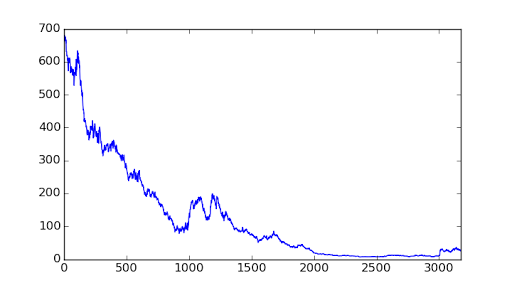
\includegraphics[width=\textwidth]{images/adj_close.png}
    \caption{Plot of adjusted close price for \textit{IBM} over all time. Notice that the indices are just numbers rather than dates and the plot goes backwards in time to the right}
\end{figure}

\noindent\begin{minipage}{\linewidth}

\noindent\textit{example 4:} Plotting multiple columns is as simple as adding a more entries to the selection statement

\lstinputlisting[style=python]{code_examples/dataframes_4.py}
\end{minipage}

\subsection{Issues}
\noindent There are some issues with the data that need to be solved to effectively use it in the way we want.

\paragraph{Trading days} The NYSE only trades for a certain number of days per year, which means that indexing by dates will return some results when the exchanges were not open. This poses problems for trying to pull out certain date ranges from the dataframe.

\paragraph{Multiple stocks} One of the dataframe's powers is to be able to contain multiple ranges, which means that we need to be able to retrieve multiple datasets and store them into the dataframe.

\paragraph{Date order} The data in the Yahoo CSV are in reverse chronological order (most recent at the top), so any analysis on the dataframe will be going backwards in time, which is not ideal.

\subsection{Solution to the issues}
\noindent To solve the trading days problem, we'll use an \ac{etf} called \textit{SPY} (S\&P 500) to serve as a basis for what days the stock market is open. The only days that exist in the dataset for this \ac{etf} are the days the stock market traded, so if we use this as a reference and use joining on the dataframes, we can recover data on only the days which had trading.\\

\noindent\begin{minipage}{\linewidth}
\noindent\textit{example 5:} Using joins to get only traded days

\lstinputlisting[style=python,firstline=1,lastline=7]{code_examples/dataframes_5.py}
\end{minipage}

\noindent If we were to print out df1, the output would be:
\begin{lstlisting}[style=python]
Empty DataFrame
Columns: []
Index: [2010-01-22 00:00:00, 2010-01-23 00:00:00, 2010-01-25 00:00:00, 2010-01-26 00:00:00]
\end{lstlisting}

\noindent This empty dataframe will be the basis for the data we want to retrieve.

\noindent The next step is to join this dataframe with a dataframe with the data for \textit{SPY}. This will keep only indices of the \textit{SPY} dataframe that also exist in the empty one.\\

\noindent\begin{minipage}{\linewidth}
\noindent\textit{example 6:} Reading in the new dataframe and joining them

\lstinputlisting[style=python,firstnumber=8,firstline=8,lastline=11]{code_examples/dataframes_5.py}
\end{minipage}

\noindent\begin{minipage}{\linewidth}
\noindent The output would now be:
\begin{lstlisting}[style=python]
				Adj Close
2010-01-22		104.34
2010-01-23		NaN
2010-01-24		NaN
2010-01-25		104.87
2010-01-26		104.43
\end{lstlisting}
\end{minipage}

\noindent To get rid of the "NaN"s, you can call \textit{dropna()} on the newly joined dataframe, but there is a better way of joining them such that the "NaN"s don't appear in the first place. The join type is called an \textit{inner} join, which joins at the intersection of the two dataframes. This way, only the dates which are in both will be kept as indices. Everything else will be thrown away.\\

\noindent\begin{minipage}{\linewidth}
\noindent\textit{example 7:} The inner join

\lstinputlisting[style=python,firstline=16,lastline=16]{code_examples/dataframes_5.py}
\end{minipage}

\subsection{Multiple stocks}
\noindent Reading in multiple stocks is as easy as just adding a for loop:\\

\noindent\begin{minipage}{\linewidth}
\noindent\textit{example 8:} Reading in multiple stocks into a single dataframe

\lstinputlisting[style=python,firstline=19,lastline=28]{code_examples/dataframes_5.py}
\end{minipage}

\noindent\begin{minipage}{\linewidth}
\noindent Here's an example of reading and plotting multiple stocks' closing price on one plot\\
\noindent\textit{example 9:} Reading and plotting multiple stocks

\lstinputlisting[style=python,firstline=31,lastline=77]{code_examples/dataframes_5.py}
\end{minipage}

\begin{figure}
	\centering
	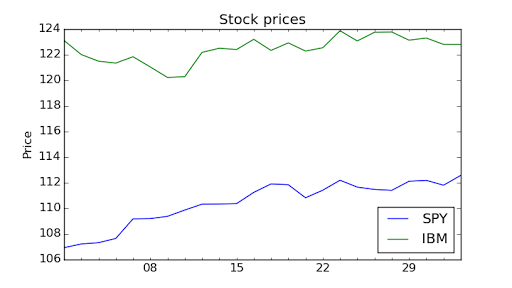
\includegraphics[width=\textwidth]{images/adj_close_mar.png}
    \caption{Plot of adjusted close price for \textit{IBM} and \textit{spy} over the month of April 2010}
\end{figure}

\subsection{Normalizing}
\noindent Sometimes when plotting, the values of a stock will be significantly different from the other stocks such that it becomes difficult to tell some of them apart. Normalizing the data allows all of them to start at the same point and then show divergences from the initial point, making it easier to compare them at the same time.\\

\noindent Normalizing the dataframe is as simple as dividing the entire dataframe by its first row
\noindent\begin{minipage}{\linewidth}
\noindent\textit{example 10:} Normalizing a dataframe

\lstinputlisting[style=python,firstline=81,lastline=83]{code_examples/dataframes_5.py}
\end{minipage}

\begin{figure}[h]
	\centering
	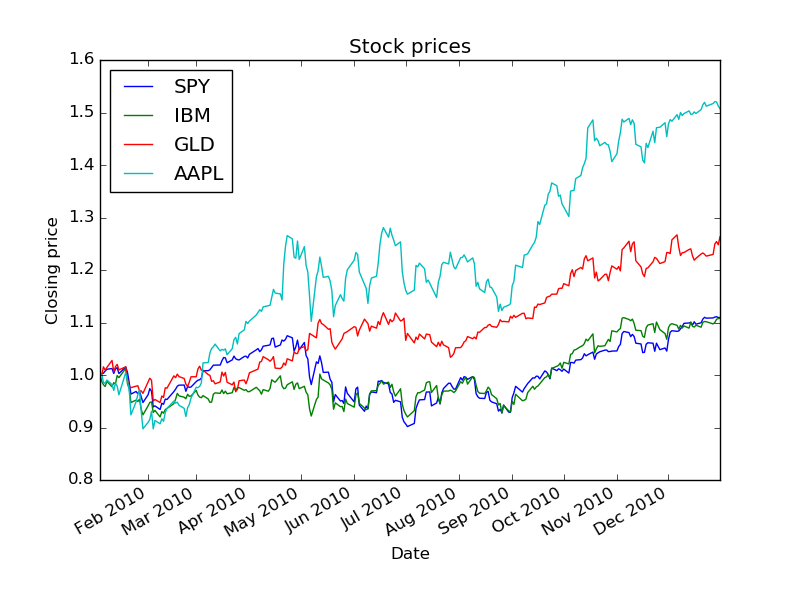
\includegraphics[width=\textwidth]{images/adj_close_normalized.png}
    \caption{Normalized stock prices over the year 2010}
\end{figure}
\newpage

\section{NumPy}

\noindent The actual data in the dataframe is actually an \textit{ndarray} in NumPy (A multidimensional homogeneous array). That means we can do operations on the data using NumPy. For example, if you have a dataframe \textit{df1}, the \textit{ndarray} would be extracted by doing

\begin{lstlisting}[style=python]
nd1 = df1.values
\end{lstlisting}

\noindent Accessing a cell in the array is as simple as:

\begin{lstlisting}[style=python]
val = nd1[row,col]
\end{lstlisting}

\noindent You can also access subarrays by indexing with the colon:

\begin{lstlisting}[style=python]
sub = nd1[0:3,1:3]
\end{lstlisting}

\noindent would capture the rectangular subarray from the first to the third rows and the second to third columns.

\paragraph{Indexing} Note that the second part of the index is 1 past the actual index that will be the last, so 0:3 only pulls out 0,1, and 2.

\noindent Like in MATLAB, you can pull out everything using just the colon. For example:

\begin{lstlisting}[style=python]
sub = nd1[3,:]
\end{lstlisting}

\noindent would retrieve all columns of row 3.

\paragraph{Negative indexing} To get the last index, you can use negative numbers (the last index would be -1, second to last -2, etc.)

\begin{lstlisting}[style=python]
sub = nd1[-1,1:3]
\end{lstlisting}

\noindent would get columns 1,2 of the last row.

\paragraph{Boolean indexing/masking} Suppose we want to get the values in an array, $a$, which are all less than the mean. NumPy's masking feature makes it really intuitive, as all you need to do is:

\begin{lstlisting}[style=python]
lessThanMean = a[a<a.mean()]
\end{lstlisting}

\noindent The array $a < a.mean()$ would be a boolean array, which might look like
\begin{lstlisting}[style=python]
[[True, True, False, False]]
\end{lstlisting}

\paragraph{Assignment} Assigning values in an array is easy using the NumPy notation. For example, say we wanted to replace the values in the first 2x2 square of \textit{nd1} with the 2x2 square in nd2 with columns 2 and 3, and rows 3, and 4. The operation would be:

\begin{lstlisting}[style=python]
nd1[0:2,0:2] = nd2[-2:,2:4]
\end{lstlisting}

\paragraph{Creating an array} Creating a numpy array is as easy as passing in a normal python list into the array method:

\begin{lstlisting}[style=python]
import numpy as np

print np.array([1,2,3])
\end{lstlisting}

\noindent Creating a 2D $mxn$ array is as simple as passing in a $m$-long list of $n$-tuples.

\begin{lstlisting}[style=python]
import numpy as np

print np.array([(1,2,3),(4,5,6)])
\end{lstlisting}

\noindent would output

\begin{lstlisting}[style=python]
[[1,2,3]
 [4,5,6]]
\end{lstlisting}

\paragraph{More initializers} You can also create arrays with certain initial values.

\begin{lstlisting}[style=python]
np.empty((5,3,2))
\end{lstlisting}

\noindent initializes an "empty" $5x3x2$ dimensional array. The values in the array are actually whatever was in the memory locations of the array pointers, so the output could look like garbage.

\begin{lstlisting}[style=python]
np.ones((5,4), dtype=np.int)
\end{lstlisting}

\noindent creates a $5x4$ array, where the value in each cell is the integer 1.

\begin{lstlisting}[style=python]
np.random.random((5,4))
\end{lstlisting}

\noindent creates a $5x4$ array with random numbers from a uniform distribution in [0.0,1.0). An example result could be:

\begin{lstlisting}[style=python]
[[ 0.82897637  0.36449978  0.91209931  0.96307279]
 [ 0.63777312  0.24482194  0.5817991   0.18043012]
 [ 0.85871221  0.98874123  0.68491831  0.53831711]
 [ 0.52908238  0.81083147  0.97440602  0.81032768]
 [ 0.98566222  0.38902445  0.16922005  0.0873198 ]]
\end{lstlisting}

\noindent Other methods or fields, such as $sum()$ or $size$ can be looked up in online documentation.
\chapter{Statistical Analysis of Time Series Data}

\noindent Pandas makes it simple to perform statistical analysis on dataframes, which is extremely important in determining different indicators and acting as inputs to the learning algorithms.\\

\section{Global statistics}
\noindent For example, if you had a dataframe $df1$ which had the closing prices for various stocks over a given time period, you can retrieve an ndarray with the mean of the columns by just calling $df1.mean()$.

\begin{figure}[h]
\begin{lstlisting}[style=python]
SPY     126.396777
IBM     166.380238
GLD     145.029775
AAPL    399.498435
XOM      77.054682
dtype: float64
\end{lstlisting}
\caption{Example output array for $mean()$ (called on closing prices for January 2010 through December 2012)}
\end{figure}

\noindent In addition to $mean$, there around 32 other global statistics that are available in pandas.

\section{Rolling statistics}

\noindent Instead of doing analysis on the entire dataset, you might want to do a rolling analysis, which only looks at certain snapshots of the data to sample. For example, you could have a 20-day moving mean, which you would calculate day-by-day by averaging the last 20 days' data. In later sections, this moving average will be explained in more detail, but some critical points of interest are when the moving average crosses the data.

\subsection{Bollinger bands\textsuperscript{\textregistered}}

\noindent Some analysts believe that significant deviations from the moving mean will result in movement back towards the mean. If the price dips far below the mean, then it might be a buy signal, whereas if it goes too high, it could indicate a time to sell. Bollinger bands are a way of measuring this deviation.\\

\noindent Bollinger observed that if you look at the volatility of the stock, and if it's too large, then you discard the movements above and below the mean, but if it's not, then it might be worth paying attention to.\\

\noindent What he did was place two new moving means, one $2\sigma$ above, and another $2\sigma$ below the moving average. If you look at deviations near to $2\sigma$, then they're worth paying attention to. If the price drops \textit{below} $2\sigma$, and then rises back up through it, then it could be a buy signal. (the price is moving back towards the average).\\

\noindent Conversely, if the price rises above $2\sigma$, then falls back down, it could be a sell signal.

\subsection{Computing rolling statistics in pandas}
\noindent Pandas provides some methods to easily calculate rolling mean ($rolling\_mean()$) and rolling standard deviation ($rolling\_std$).\\

\noindent\begin{minipage}{\linewidth}

\noindent\textit{example 11:} Calculating a 20-day rolling mean

\lstinputlisting[style=python,firstline=37,lastline=37]{code_examples/statistics_1.py}
\end{minipage}

\begin{figure}[h!]
	\centering
	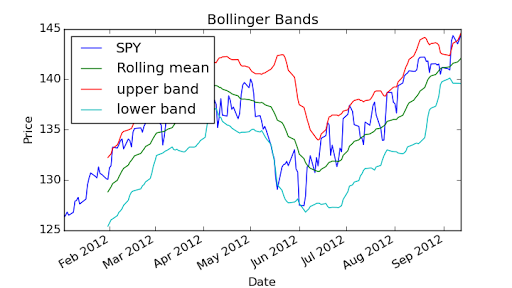
\includegraphics[width=\textwidth]{images/bollinger_bands.png}
    \caption{Plot of rolling mean for \textit{SPY} with Bollinger bands\textsuperscript{\textregistered}}
\end{figure}
\newpage

\noindent The Bollinger bands\textsuperscript{\textregistered} were calculated as follows:\\

\noindent\textit{example 12:} Calculating bollinger bands

\lstinputlisting[style=python]{code_examples/statistics_1.py}

\section{Daily returns}
\noindent Daily returns are how much a stock's price went up or down on a given day. They are an extremely important statistic as they can be a good comparison between different stocks.

\begin{equation*}
	daily\_ret[t] = \frac{price[t]-price[t-1]}{price[t-1]} = \frac{price[t]}{price[t-1]}-1
\end{equation*}

\begin{lstlisting}[style=python]
daily_ret = (df / df.shift(1).values) - 1
daily_ret.ix[0,:] = 0
\end{lstlisting}

\begin{figure}[h!]
	\centering
	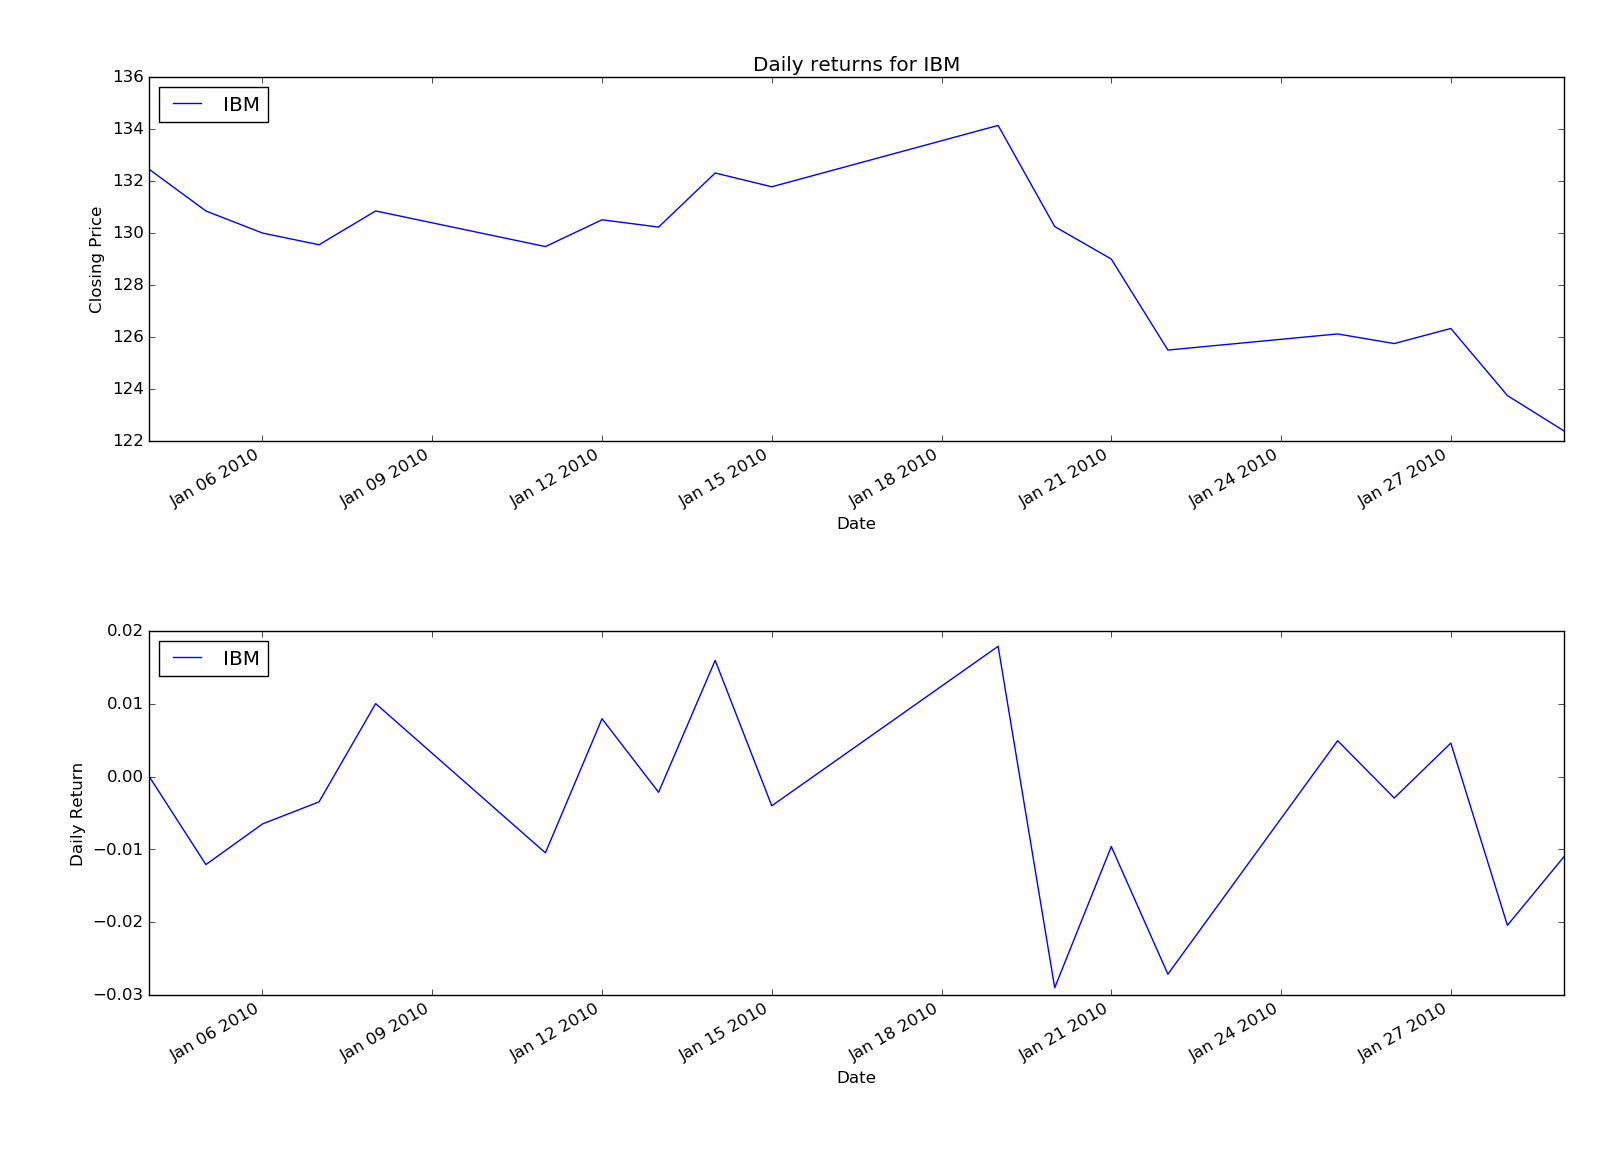
\includegraphics[width=\textwidth]{images/daily_returns.png}
    \caption{Plot of \textit{IBM}'s prices (top) with daily returns (bottom)}
\end{figure}

\section{Cumulative Returns}
\noindent Cumulative return is calculated by finding the gain from the beginning of the range to the current time, i.e.

\begin{equation*}
	cum\_ret[t] = \frac{price[t]}{price[0]}-1
\end{equation*}

\noindent For example, if the price at the beginning was \$125, and the current price is \$142, then the gain/cumulative return is $\frac{142}{125}-1 = .136 (13.6\%)$\\

\noindent Cumulative returns are essentially the original dataset normalized.

\section{Incomplete data}
\noindent People assume that financial data is extremely well-documented and that perfect data is recorded minute by minute. They also believe that there are no gaps or missing data points. However, for any particular stock, it might have different prices on different stock exchanges! It's difficult to know who's right all the time. Also, not all stocks trade every day (they might suddenly start trading or stop trading).\\

\noindent You might think you can just interpolate the data between breaks, but that'd cause statistical errors and a side-effect of "looking into the future" when doing analysis on that subset of data. The better way of doing it to minimize error is to fill forward and backwards.

\subsection{Filling}
\noindent To fix the "NaN"/empty data, you can use filling to maintain the last known value until known data is reached. For example, if you had a stock that didn't have data until 2001 and then stopped having data in 2006 but then started having data again in 2012, you could fill forward from 2006-2012 and then fill backwards from 2001 back to whenever you want your data to start.\\

\noindent\begin{minipage}{\linewidth}

\noindent\textit{example 13:} Filling in missing data using $fillna()$
\begin{lstlisting}[style=python]
df = get_data(symbols,dates)

df.fillna(method="ffill",inplace=True)
df.fillna(method="bfill",inplace=True)
\end{lstlisting}
\end{minipage}

\begin{figure}[h!]
	\centering
	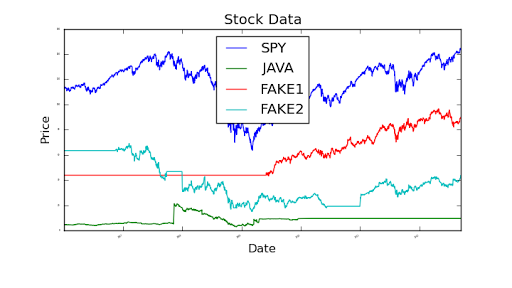
\includegraphics[width=\textwidth]{images/filled_data.png}
    \caption{Data will forward and backwards filled values (horizontal lines)}
\end{figure}
\newpage

\section{Histograms and scatter plots}
\noindent It's difficult to draw conclusions directly from daily returns plots, so histograms make it easier to see what's going on. A histogram allows you to see how many occurrences of each return happens relative to other returns. This histogram typically follows a Gaussian over large periods of time.\\

\subsection{Histograms}

\noindent From the histogram we can determine a few key statistics: mean, standard deviation, and kurtosis. Kurtosis is a measure of how close the curve is to a Gaussian. In stock data, there are usually more occurrences at high deviations (causing sort of "fat tails"), which would be reflected as a positive kurtosis. Skinny tails would mean a negative kurtosis.

\begin{figure}[h!]
	\centering
	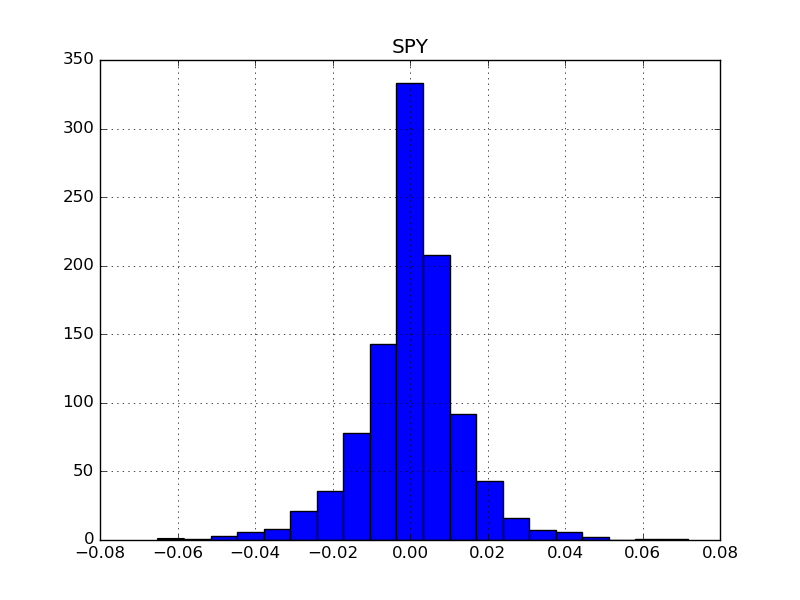
\includegraphics[width=\textwidth]{images/histograms_1.png}
    \caption{Histogram of daily returns \textit{SPY} from January 2009 through December 2012}
\end{figure}
\newpage

\noindent\begin{minipage}{\linewidth}
\noindent\textit{example 14:} Getting a histogram
\noindent The histogram above was generated by just calling $hist()$ on the daily returns dataframe as such:

\begin{lstlisting}[style=python]
daily_returns.hist(bins=20)
\end{lstlisting}
\end{minipage}

\noindent The $bins$ parameter is essentially the resolution of the histogram. The domain is divided into 20 bins and anything within those bins counts for that bin's count in the histogram.

\noindent Other statistics like mean and standard deviation are easily calculated:

\noindent\begin{minipage}{\linewidth}
\begin{lstlisting}[style=python]
mean = daily_returns['SPY'].mean()
print "mean=",mean

std = daily_returns['SPY'].std()
print "std deviation=",std
\end{lstlisting}
\end{minipage}

\noindent\begin{minipage}{\linewidth}
\noindent Which outputs:
\begin{lstlisting}[style=python]
mean= 0.000509326569142
std deviation= 0.0130565407719
\end{lstlisting}
\end{minipage}

\noindent\begin{minipage}{\linewidth}
\noindent We can now plot the mean and standard deviations on the plot to make analysis easier:
\begin{lstlisting}[style=python]
plt.axvline(mean,color='w',linestyle='dashed',linewidth=2)
plt.axvline(mean+std,color='r',linestyle='dashed',linewidth=2)
plt.axvline(mean-std,color='r',linestyle='dashed',linewidth=2)
\end{lstlisting}
\end{minipage}

\begin{figure}[h!]
	\centering
	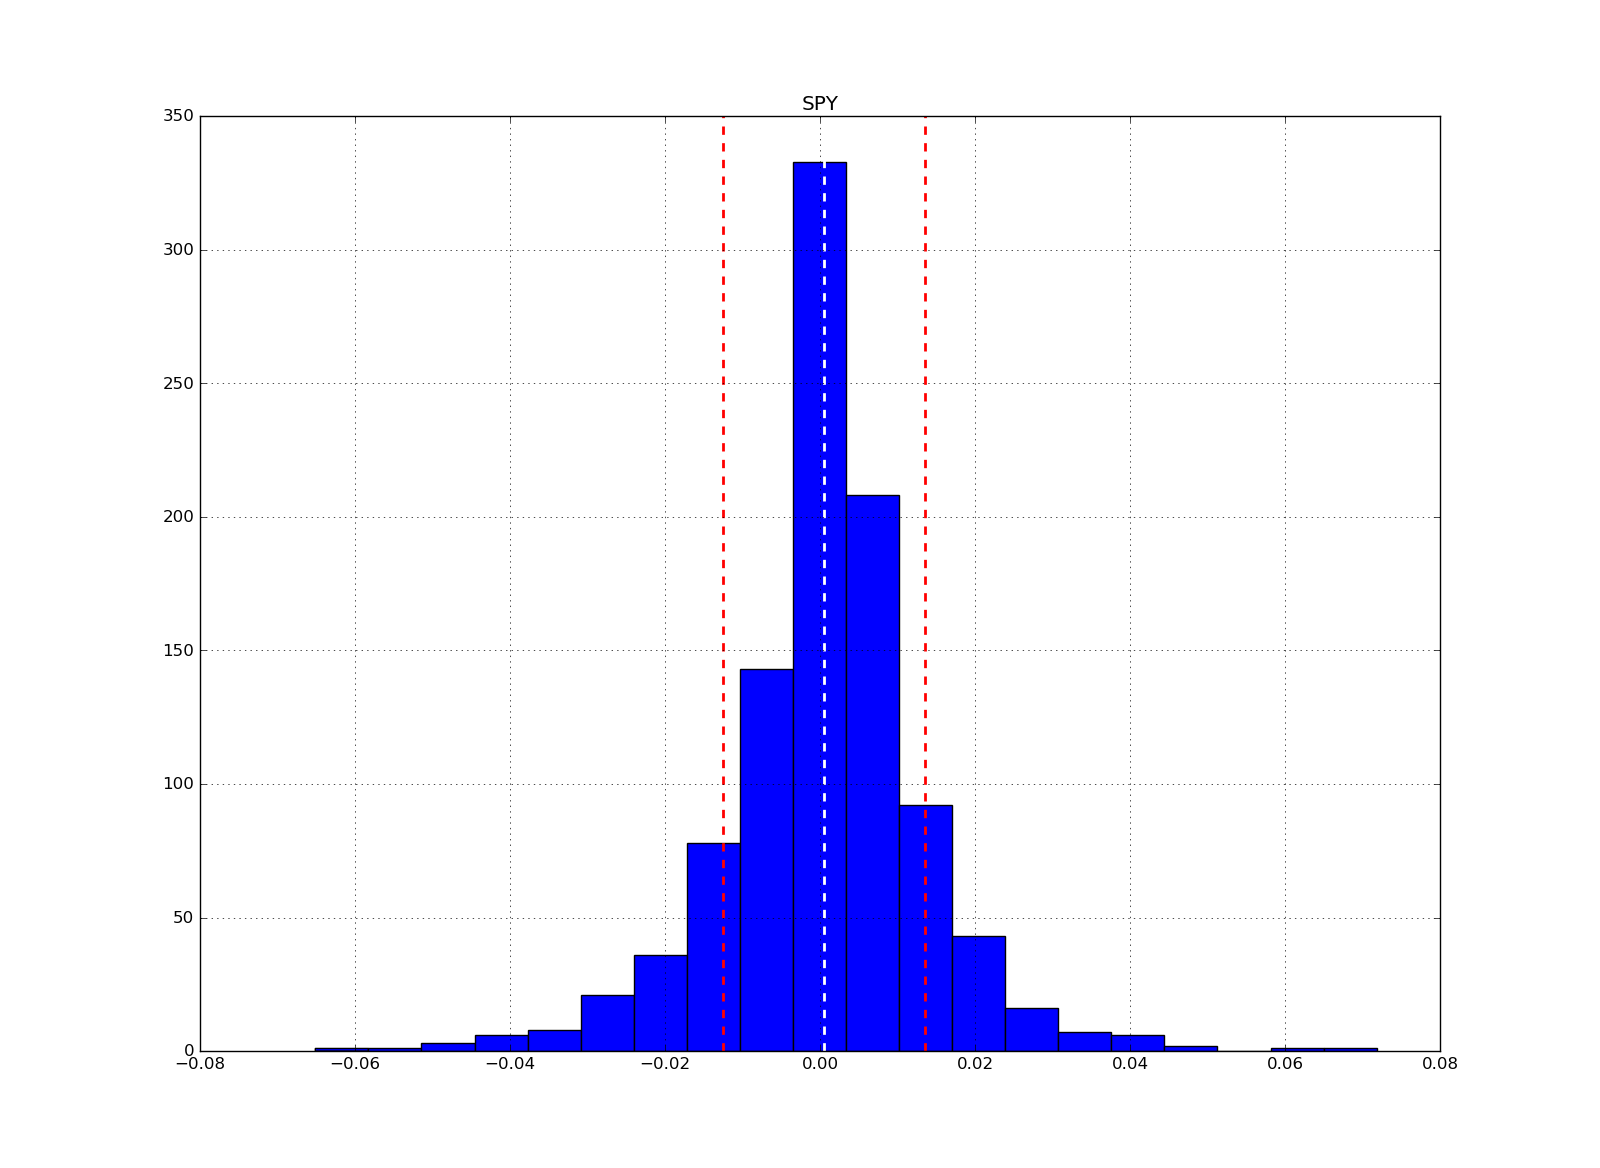
\includegraphics[width=\textwidth]{images/histograms_2.png}
    \caption{Histogram with mean (white) and $1\sigma$ (red) plotted}
\end{figure}

\noindent\begin{minipage}{\linewidth}
\noindent The output of
\begin{lstlisting}[style=python]
print daily_returns.kurtosis()
\end{lstlisting}
\end{minipage}

\noindent\begin{minipage}{\linewidth}
\noindent is:
\begin{lstlisting}[style=python]
SPY    3.376644
\end{lstlisting}
\end{minipage}

\noindent which means that the data has fat tails since it's positive.\\

\noindent The utility of these histograms comes when plotting them together. It's easy to compare multiple stocks in terms of their returns and volatility. If stock A's curve is skewed more positive and is thinner than stock B, then it has a low volatility with higher returns vs stock B.\\

\begin{figure}[h!]
	\centering
	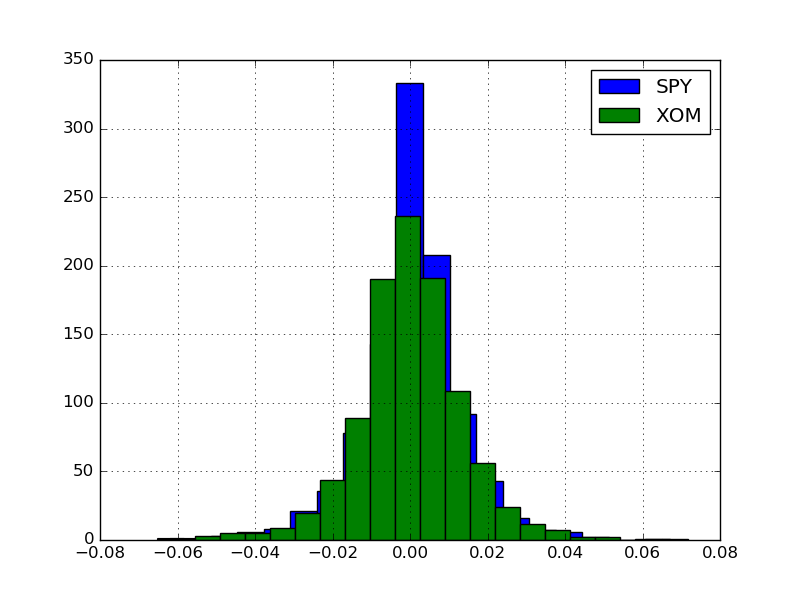
\includegraphics[width=\textwidth]{images/histograms_comparison.png}
    \caption{Histogram comparison of \textit{SPY} and \textit{XOM}}
\end{figure}
\newpage
\noindent By looking at this chart, you can see that \textit{SPY} and \textit{XOM} are about the same in volatility ($\sigma_{SPY} = .013057, \sigma_{XOM} = .013647$). However, \textit{SPY} would have higher returns since $\overline{R_{SPY}} = .000509$ whereas $\overline{R_{XOM}} = .000151$ 

\subsection{Scatter plots}
\noindent Scatter plots are another way of visualizing the correlation between two stocks. Say you had a dataframe with the daily returns for \textit{SPY} and \textit{XYZ}. If you took just the $ndarray$ containing the y-axis values, and then plotted \textit{SPY} on the x-axis and \textit{XYZ} on the y-axis, you would see a bunch of points that might have a certain trend.\\

\noindent If you take a linear regression of this data, the slope would be called the beta ($\beta$) value. If the $\beta$ value for \textit{SPY} and \textit{XYZ} is 1, it means that, on average, if \textit{SPY} (the market) moves up by 1\%, then \textit{XYZ} also moves up by 1\%.\\

\noindent The y-intercept of the line is called $\alpha$. It describes how the stock on the y-axis performs with respect the stock on the x-axis. If the $\alpha$ value of \textit{XYZ} with respect to \textit{SPY} is positive, then, on average, \textit{XYZ} is returning more than the market overall.

\paragraph{Correlation} If there isn't any correlation in the dataset, then the linear regression doesn't tell you anything about the relationship. A common method for calculating the correlation is by finding the \textit{sample Pearson correlation coefficient, $r_{xy}$}. It's calculated by the following:

\begin{equation*}
	r_{xy} = \frac{cov(X,Y)}{\sigma_{X}\sigma_{Y}} = \frac{\sum_{i=1}^{n}(x_i - \bar{x})(y_i - \bar{y})}{\sqrt{\sum_{i=1}^{n}(x_i - \bar{x})^2}\sqrt{\sum_{i=1}^{n}(y_i - \bar{y})^2}}
\end{equation*}

where $cov$ is the covariance. In this case, X would be the daily return for \textit{SPY} and Y would be the daily return for \textit{XYZ}.
\noindent If $|r_{X,Y}| = 1$, then the two are perfectly correlated (either positively or negatively, depending on the sign of $\rho$). If $|r| < 1$, then there is possible correlation, but a value closer to 1 means better correlation. If $r = 0$, there is no correlation. \\

\noindent\begin{minipage}{\linewidth}
\noindent\textit{example 15:} Plotting scatter plots, getting $\alpha$ and $\beta$ values, and determining correlation
\begin{lstlisting}[style=python]
# scatter plot for XOM vs SPY
daily_ret.plot(kind='scatter',x='SPY',y='XOM',title="Scatter plot")
beta_XOM,alpha_XOM = np.polyfit(daily_ret['SPY'],daily_ret['XOM'],1)
plt.plot(daily_ret['SPY'],beta_XOM*daily_ret['SPY']+alpha_XOM,'-',color='r')
plt.show()

# scatter plot for GLD vs SPY
daily_ret.plot(kind='scatter',x='SPY',y='GLD',title="Scatter plot")
beta_GLD,alpha_GLD = np.polyfit(daily_ret['SPY'],daily_ret['GLD'],1)
plt.plot(daily_ret['SPY'],beta_GLD*daily_ret['SPY']+alpha_GLD,'-',color='r')
plt.show()

print "Beta XOM: ", beta_XOM
print "Alpha XOM: ",alpha_XOM
print "Beta GLD: ",beta_GLD
print "Alpha GLD: ",alpha_GLD

# calculate correlation using pearson method
print "Correlation matrix: \n", daily_ret.corr(method='pearson')
\end{lstlisting}
\end{minipage}
\noindent which outputs:
\begin{lstlisting}[style=python]
Beta XOM:  0.85753872112
Alpha XOM:  -0.000285580653638
Beta GLD:  0.0663816850634
Alpha GLD:  0.000660583984316
Correlation matrix: 
          SPY       XOM       GLD
SPY  1.000000  0.820423  0.074771
XOM  0.820423  1.000000  0.079401
GLD  0.074771  0.079401  1.000000
\end{lstlisting}

\noindent Looking at the $\beta$ values, you can see that \textit{XOM} is more responsive to market changes, while \textit{GLD} is relatively unresponsive. However, \textit{GLD} tends to perform better than the market on average, since its $\alpha$ is positive.\\

\noindent But these values are meaningless without seeing what their correlations are. Looking at the correlation matrix, \textit{XOM} is pretty well correlated with \textit{SPY}, whereas \textit{GLD} has a very low correlation, so changes \textit{GLD} aren't really correlated with changes in the market.

\begin{figure}[h!]
	\centering
    \subcaptionbox{\textit{XOM}}[.45\linewidth]{
    	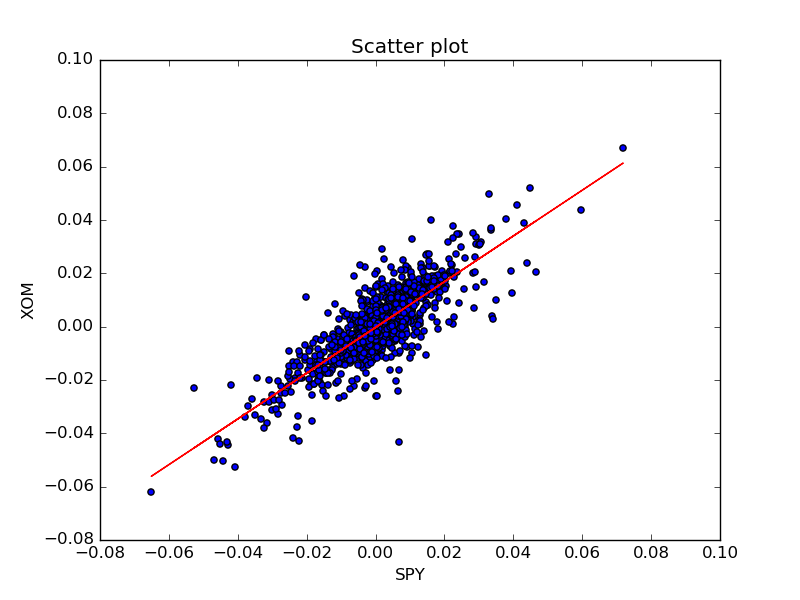
\includegraphics[width=.5\linewidth]{images/scatter_XOM.png}
    }
    \subcaptionbox{\textit{GLD}}[.45\linewidth]{
    	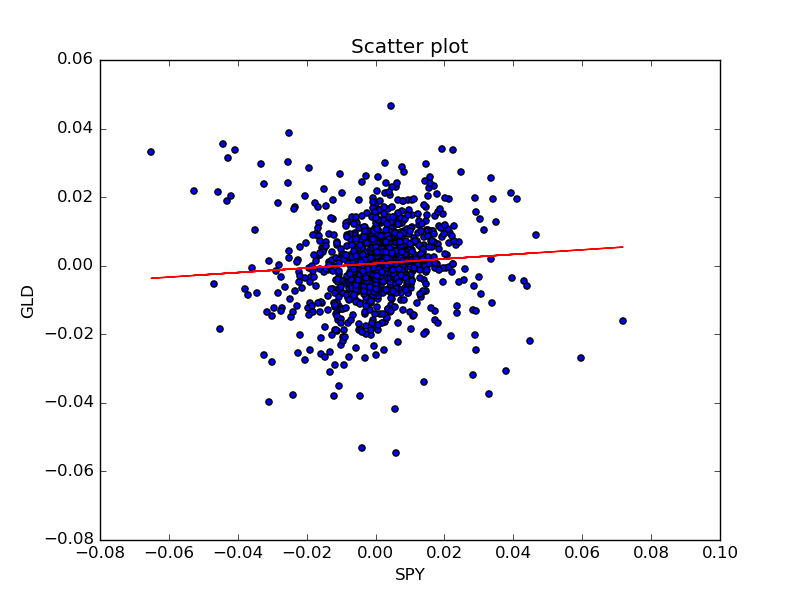
\includegraphics[width=.5\linewidth]{images/scatter_GLD.png}
    }
    \caption{Scatter plots for \textit{XOM} and \textit{GLD}}
\end{figure}
\newpage

\noindent Looking at the plots, it's easy to see that the points for \textit{XOM} are more correlated and match the line better than do those of \textit{GLD}.

\section{Sharpe ratio and other portfolio statistics}

\noindent The \textbf{portfolio} is the collection of all stocks currently owned by a person. It's important to know various statistics associated with the portfolio to make informed decisions on what to sell/buy.

\noindent Suppose you begin with a portfolio $p$ consisting of the following parameters:
\begin{lstlisting}[style=python]
start_val = 1000000
start_date = '2009-01-01'
end_date = '2011-12-31'
symbols = ['SPY','XOM','GOOG','GLD']
allocs = [0.4, 0.4, 0.1, 0.1] # @ beginning, 40% to SPY, 40% to XOM, etc
\end{lstlisting}

\noindent Now suppose we want to find the value of this portfolio day-by-day. If we normalize the portfolio dataframe, we essentially have a dataframe containing cumulative returns for each index. If we multiply this by $allocs$, we get returns scaled by each percentage of the total portfolio. Then, multiply by $start\_val$ to get each stock's total value. Finally, take the sum of this penultimate dataframe to get a single-column dataframe with the total portfolio value at each point in time. In Python,

\noindent\begin{minipage}{\linewidth}
\begin{lstlisting}[style=python]
# get cumulative returns
df = get_data(symbols,pd.date_range(start_date,end_date))
df = normalize(df)

# get changes for each stock by their percentages of the starting value
alloced = df*allocs

# get dollar value of changes
vals = alloced*start_val

# sum to get total value
portfolio_value = vals.sum(axis=1)
\end{lstlisting}
\end{minipage}

\noindent We may now compute various statistics on the portfolio's value.

\paragraph{Daily returns} Obviously, daily returns of the entire portfolio would be an important statistic, as they indicate how the portfolio changes over time. For some statistics, we need to get rid of the 0 at the beginning of the daily return or else it'll throw off the values.

\begin{lstlisting}[style=python]
daily_rets = daily_rets[1:]
\end{lstlisting}

\paragraph{Cumulative returns} The total cumulative return of the portfolio is another interesting statistic, as you can see if the overall gain was positive or negative.
\begin{lstlisting}[style=python]
cum_ret = (port_val[-1]/port_val.ix[0,:]) - 1
\end{lstlisting}

\paragraph{Avg. and Std. Deviation} These two are the main statistics that get thrown off by the 0 at the beginning. If it were there, the mean would be closer to 0, even though technically 0 isn't actually one of the returns.

\begin{lstlisting}[style=python]
avg_daily_ret = daily_rets.mean()
std_daily_ret = daily_rest.std()
\end{lstlisting}

\subsection{Sharpe Ratio}
\noindent The \textbf{Sharpe Ratio} is a metric that adjusts return for risk. It enables a quantitative way to compare two stocks in terms of their returns and volatility. The Sharpe Ratio is calculated based on the assumption that, \textit{Ceteris paribus}\footnote{all else held equal},
\begin{itemize}
	\item Lower risk is better
    \item Higher return is better
\end{itemize}
Being an economic indicator, it also takes into account the opportunity cost/return of putting the money in a risk-free asset such as a bank account with interest.

\noindent A sort of risk-adjusted return may be calculated as follows:
\begin{equation*}
	R_{adj} = \frac{R_p - R_f}{\sigma_p}
\end{equation*}
where $R_p$ is the portfolio return, $R_f$ is the risk-free rate of return, and $\sigma_p$ is the volatility of the portfolio return.

\noindent This ratio is a sort of basis for how the Sharpe Ratio is calculated. The Sharpe Ratio is as follows:

\begin{equation*}
	S = \frac{E[R_p - R_f]}{std(R_p-R_f)}
\end{equation*}

\noindent Since we're looking at past data, the expected value is actually the mean of the dataset, so this becomes:\\

\begin{equation*}
	S = \frac{\overline{(R_p - R_f)}}{std(R_p-R_f)}
\end{equation*}

\noindent One question is where $R_f$ comes from. There are three main ways of getting the data for the risk-free rate:
\begin{enumerate}
	\item The London Inter-Bank Offer Rate (LIBOR)
	\item The interest rate on the 3-month Treasury bill
    \item 0\% (what people have been using recently...)
\end{enumerate}

\noindent LIBOR changes each day, and the Treasury bill changes slightly each day, but interest in bank accounts are typically paid in 6-month or yearly intervals. Using this simple trick, you can convert the annual/biannual amount to a daily amount:\\

\noindent Suppose the yearly interest rate is $I$. If we start at the beginning of the year with a value $P$, the new value after interest is paid will be $P'$. To find the equivalent daily interest value, $I_{eq}$,

\begin{align*}
	P' &= P(1+I_{eq})^{252}\\
    P(1+I) &= P(1+I_{eq})^{252}\\
    1+I &= (1+I_{eq})^{252}\\
    (1+I_{eq}) &= \sqrt[\leftroot{-2}\uproot{2}252]{1+I}\\
    I_{eq} &= \sqrt[\leftroot{-2}\uproot{2}252]{1+I} - 1
\end{align*}

\noindent Therefore, $R_f$, the daily risk-free rate, is just $\sqrt[\leftroot{-2}\uproot{2}252]{1+I} - 1$. The reason it's 252 instead of 365 is because there are only 252 trading days in a year.\\

\noindent Since we're treating $R_f$ as constant, the standard deviation in the denominator just becomes $std(R_p)$, so the final equation for the Sharpe Ratio becomes:

\begin{equation*}
	S = \frac{\overline{(R_p - R_f)}}{\sigma_{R_p}}
\end{equation*}

\paragraph{Sampling rate} The Sharpe Ratio can vary widely depending on the sampling frequency. Since SR is an annual measure, any calculations that are done with samples more frequent than yearly need to be scaled to get the annual ratio. To adjust the calculated Sharpe Ratio to be "annualized", you just multiply by a factor of $\sqrt{\# samples\ per\ year}$. So if you sample daily, the Sharpe Ratio would become:

\begin{equation*}
	S = \frac{\overline{(R_p - R_f)}}{\sigma_{R_p}}\sqrt{252}
\end{equation*}

\noindent\textit{example:} Given 60 days of data with the following statistics:\\
\noindent$R_p = 10 bps$\\
$R_f = 2 bps$\\
$\sigma_{R_p} = 10 bps$,\\
what is the Sharpe Ratio? One $bps$ is one hundredth of a percent.

\begin{equation*}
	S = \frac{\overline{(R_p - R_f)}}{\sigma_{R_p}} = \frac{10-2}{10}\sqrt{252} 
    \approx 12.70
\end{equation*}

\section{Optimizers}
\noindent An optimizer can:
\begin{itemize}
  \item Find minimum/maximum values of functions
  \item Build parameterized models based on data
  \item Refine allocations to stocks in portfolios
\end{itemize}

\noindent For example, say you have the function $f(x) = (x-1.5)^2 + .5$, and you want to find the minimum. It's trivial to use calculus and find the minimum analytically, but you can't always do so if you don't have an analytical model of the data. Let's put this in Python:

\noindent\begin{minipage}{\linewidth}
\begin{lstlisting}[style=python]
import pandas as pd
import matplotlib.pyplot as plt
import numpy as np
import scipy.optimize as spo

def f(x):
	y = (x-1.5)**2 + .5
	print "x = {}, y = {}".format(x,y)
	return y
    
def test_run():
 	guess = 2.0
	min_result = spo.minimize(f, guess, method='SLSQP', options={'disp':True})
	print "minima found at:"
	print "x = {}, y = {}".format(min_result.x,min_result.fun)
    
if __name__ == "__main__":
	test_run()
\end{lstlisting}
\end{minipage}

\noindent\begin{minipage}{\linewidth}
\noindent outputs:
\begin{lstlisting}[style=python]
x = [ 2.], y = [ 0.75]
x = [ 2.], y = [ 0.75]
x = [ 2.00000001], y = [ 0.75000001]
x = [ 0.99999999], y = [ 0.75000001]
x = [ 1.5], y = [ 0.5]
x = [ 1.5], y = [ 0.5]
x = [ 1.50000001], y = [ 0.5]
Optimization terminated successfully.    (Exit mode 0)
            Current function value: [ 0.5]
            Iterations: 2
            Function evaluations: 7
            Gradient evaluations: 2
minima found at:
x = [ 1.5], y = [ 0.5]
\end{lstlisting}
\end{minipage}

\begin{figure}[h!]
	\centering
	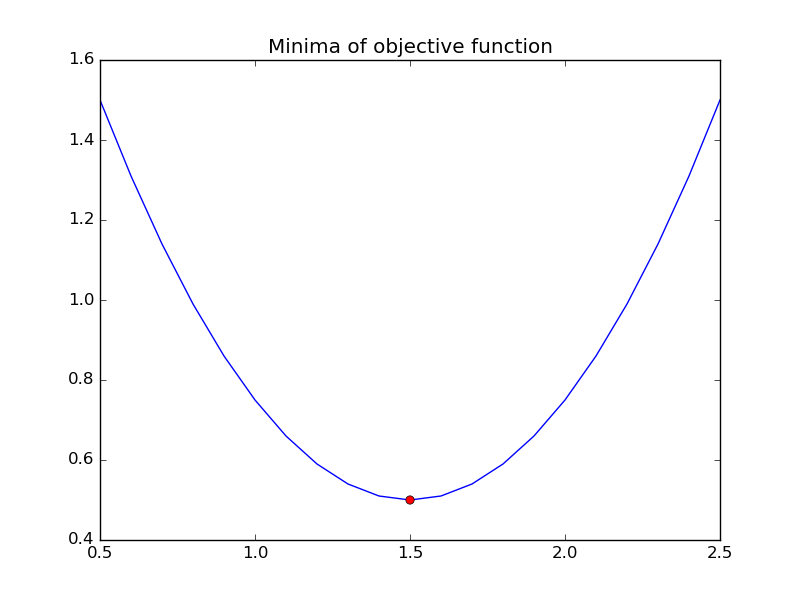
\includegraphics[width=\linewidth]{images/minima.png}
    \caption{Numerical solution to finding the minimum of $f(x) = (x-1.5)^2 + .5$}
\end{figure}
\newpage

\subsection{Pitfalls}
\noindent Optimizers aren't perfect, and since the method used above uses the gradient of the current point to move to the next point, it can be tripped up by various abnormalities in the function it's trying to minimize, such as:

\begin{itemize}
\item\textit{Flat ranges:} If a portion of the graph is flat (the slope is close to or is 0), then the solver will either take a lot of iterations to solve for the minimum or it might not ever be able to move to a new point, unless it can find a way out.
\item\textit{Discontinuities:} If there are discontinuities, the gradient might not be defined well enough for the solver to continue.
\item\textit{Multiple minima:} Say you have a function $f(x) = x^4-2x^2+x^2$. This function has 2 minima at $(0,0)\ and\ (1,0)$. If the solver starts at $x=1.5$, it'll find the minimum at $(1,0)$, but it won't ever reach the other minimum. Conversely, if the solver starts at $x=-1.5$, it'll find the minimum at $(0,0)$. Therefore, it's easy to get trapped in a local minimum that may not be the actual \textit{global} minimum.
\end{itemize}

\subsection{Convex problems}
\noindent A real-valued function $f(x)$ defined on an interval is called \textbf{convex} if the line segment between any two points on the graph of $f(x)$ on that interval lies above the graph. Otherwise, it's called \textbf{non-convex}.

\subsection{Building a parameterized model}
\noindent If you have a set of data points representing rainfall and humidity that were gathered, you might want to find a function that best fits those points. Say you wanted to fit a line $f(x) = mx + b$ to the points. In this case, you can use linear algebra and find the least-squares solution, but you can also use an optimizer to find the \textit{best} parameters $m$ and $b$.\\

\noindent What does "best" mean? Well, we can devise a measure for the error for each point:

\begin{equation*}
	e_i = (y_i - f(x_i))^2 = (y_i - (mx_i+b))^2
\end{equation*}

\noindent which is just the difference between the actual value and our model's predicted value. The reason it's squared is to ensure that negative errors don't reduce the total error when we sum up every $e_i$. 
\begin{equation*}
	E = \sum^{n}_{i=1}(y_i - (mx_i+b))^2
\end{equation*}
\noindent Now that we have what we want to minimize, $E$, we can use a minimizer to find the best $m$ and $b$. To make the parameters nicer to work with in Python (and allow generalization to higher degrees of polynomials), we'll rename $m$ and $b$ to $C_0$ and $C_1$. Now, $f(x) = C_ox+C_1$.

\noindent\begin{minipage}{\linewidth}
\noindent\textit{example 16:}
\begin{lstlisting}[style=python]
import pandas as pandas
import matplotlib.pyplot as plt
import numpy as np
import scipy.optimize as spo

# line is a tuple (C0, C1)
def error(line, data):
	return np.sum((data[:,1] - (line[0]*data[:,0] + line[1])) ** 2)

def fit_line(data,error_func):
	# initial guess for parameters
	l = np.float32([0, np.mean(data[:,1])])

	return spo.minimize(error_func, l, args=(data,), method='SLSQP', options={'disp':True}).x

def test_run():
	original = np.float32([4,2])
	print "original line: C0 = {}, C1 = {}".format(original[0],original[1])
	Xoriginal = np.linspace(0,10,40)
	Yoriginal = original[0]*Xoriginal + original[1]

	plt.plot(Xoriginal,Yoriginal,'b--',linewidth=2.0,label="Original line")

	# add some random noise to the data
	noise_sigma = 4.0
	noise = np.random.normal(0,noise_sigma,Yoriginal.shape)
	data = np.asarray([Xoriginal,Yoriginal+noise]).T

	plt.plot(data[:,0],data[:,1], 'go', label="Data points")

	l_fit = fit_line(data,error)
	print "Fitted line: C0 = {}, C1 = {}".format(l_fit[0],l_fit[1])
	plt.plot(data[:,0],l_fit[0]*data[:,0] + l_fit[1],'r--', linewidth=2.0,label="Fitted line")

	plt.legend(loc='upper right')
	plt.show()

if __name__ == "__main__":
	test_run()
\end{lstlisting}
\end{minipage}
 the minimizer.
\begin{figure}[h!]
	\centering
	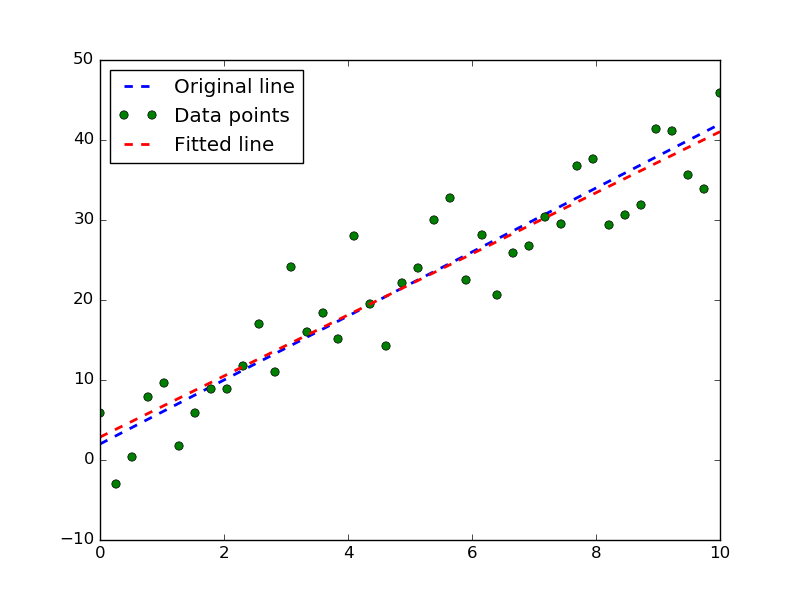
\includegraphics[width=\linewidth]{images/line_fit.png}
    \caption{Line of best fit found using parametric mininimization}
\end{figure}
\newpage

\noindent An example of extending $fit\_line$ to higher-degree polynomials can be found in the appendix.

\section{Portfolio Optimization}
\noindent Now that wee have the tools to optimize a function, we can use it to optimize our portfolio! We can choose to optimize/minimize/maximize various measures, such as daily returns, cumulative returns, or Sharpe Ratio based on the percent allocation of all of the stocks in the portfolio.

\subsection{Framing the problem}
\noindent First we need three things:
\begin{enumerate}
\item a function, $f(x)$, to minimize
\item an initial guess for $x$
\item the optimizer
\end{enumerate}

\noindent In our case, $x$ is actually the set of allocations for the stocks. Also, since we want to maximize Sharpe Ratio, we need to multiply $f(x)$ by -1 to call the minimizer.
\chapter{Essential Economics}
This chapter discusses terminology, stock market dynamics, and important indicators in economics. This will allow us to more accurately judge the value of an economic decision and make predictions on the market.

\section{Funds}

We'll discuss three different types of funds: \acf*{etf}, mutual funds, and hedge funds. Different types of funds are governed under different rules. \ac*{etf}s are similar to stocks in that they are bought and sold at will like stocks- very liquid. However, \ac*{etf}s typically represent baskets of stocks, and it is known to the trader what the fund represents. Mutual funds can only be bought and sold at the end of the day, and the holdings within a mutual fund are only disclosed every quarter. The least transparent holdings are that of a hedge fund. Before investors can buy shares in the fund, they must sign a long term agreement and holdings are rarely disclosed. \\

\subsection{About Funds}

For stocks and \ac*{etf}s, having a large "cap" means that the total value of stocks (number of stocks $\times$ price of a stock) in a company is worth many billions of dollars. Moreover, the price of a stock doesn't reflect the value of a company, but the price at which they are selling shares. \ac*{etf}s, like stocks, can easily be traded through individuals alone, whereas shares in mutual funds require a broker and hedge fund shares require more of a one on one relationship. Managers of \ac{etf}s and mutual funds are compensated based on expense ratios, which denote a percentage of \ac{aum}. For an \ac{etf}, expense ratios range from 0.01\% to 1\%, and in mutual funds from 0.5\% to 3\%. Hedge funds follow a "two and twenty" policy, where managers get 2\% of the \ac{aum} and 20\% of the profits.\\

The type of a fund can be more easily recognized by how it's named. For example, an \ac*{etf} has a ticker, or stock symbol, with three or four letters, like AAPL. A mutual fund has five letters, like VTINX, and a hedge fund doesn't have a ticker because shares are much less liquid. How much money is managed by a fund is known as the \ac{aum}, and shares represent percentages of the \ac{aum}. \\

It's fairly clear to see that hedge funds are very different from \ac{etf}s and mutual funds. Hedge funds typically have no more than 100 investors, whereas \ac{etf}s and mutual funds have thousands. Those that invest in hedge funds are typically very wealthy individuals, institutions, and funds of funds. Funds of funds typically take large sums of money from potentially many places and invest in several hedge funds. This is a bridge for smaller investors to participate in hedge fund. The goal of a hedge fund typically falls along the lines of two ideals. The hedge fund may be out to beat a bench mark which is to say that the hedge fund aims to outperform an index of stocks. A hedge fund could also aim for absolute return, which translates to net positive profit no matter what, but usually takes more time and has fewer returns as a trade off for stability. We'll be focusing on hedge funds because they are the most computationally demanding.

\subsection{Fund Metrics and Operations}
Measuring the performance of a fund is vital for making financial decisions in the market, so here we'll discuss a few. Overall success can be measured by cumulative return, which is the percentage of an original value made in a given time: $\frac{end-start}{start}$. However, this means little if the portfolio is rapidly and wildly fluctuating. Hence it's also useful to measure the volatility of a portfolio. This is simply measured by the standard deviation of daily returns; it's best to have low volatility. Another important measure is the return on risks. This is done by calculating the \ac{sr}, also called risk-adjusted reward. 
\begin{align*}
\ac{sr}=\frac{mean(\mbox{daily returns}-\mbox{risk free rate})}{\mbox{volatility}}\sqrt{252}
\end{align*}
The factor of $\sqrt{252}$ comes from the number of trading days in a year. These factors can give us an idea of how well a portfolio is performing.\\

As previously mentioned, hedge funds are very computationally intensive environments. Let's delve into the details of how a typical hedge fund works. Central to the operation of a hedge fund is its trading algorithms. Normally, a target portfolio is decided upon, then historical stock data and the target portfolio are fed to the trading algorithms to produce orders. The orders are sent to the market to alter the live portfolio, which is again fed back into trading algorithms. 
\newpage

\begin{figure}[h!]
\begin{center}
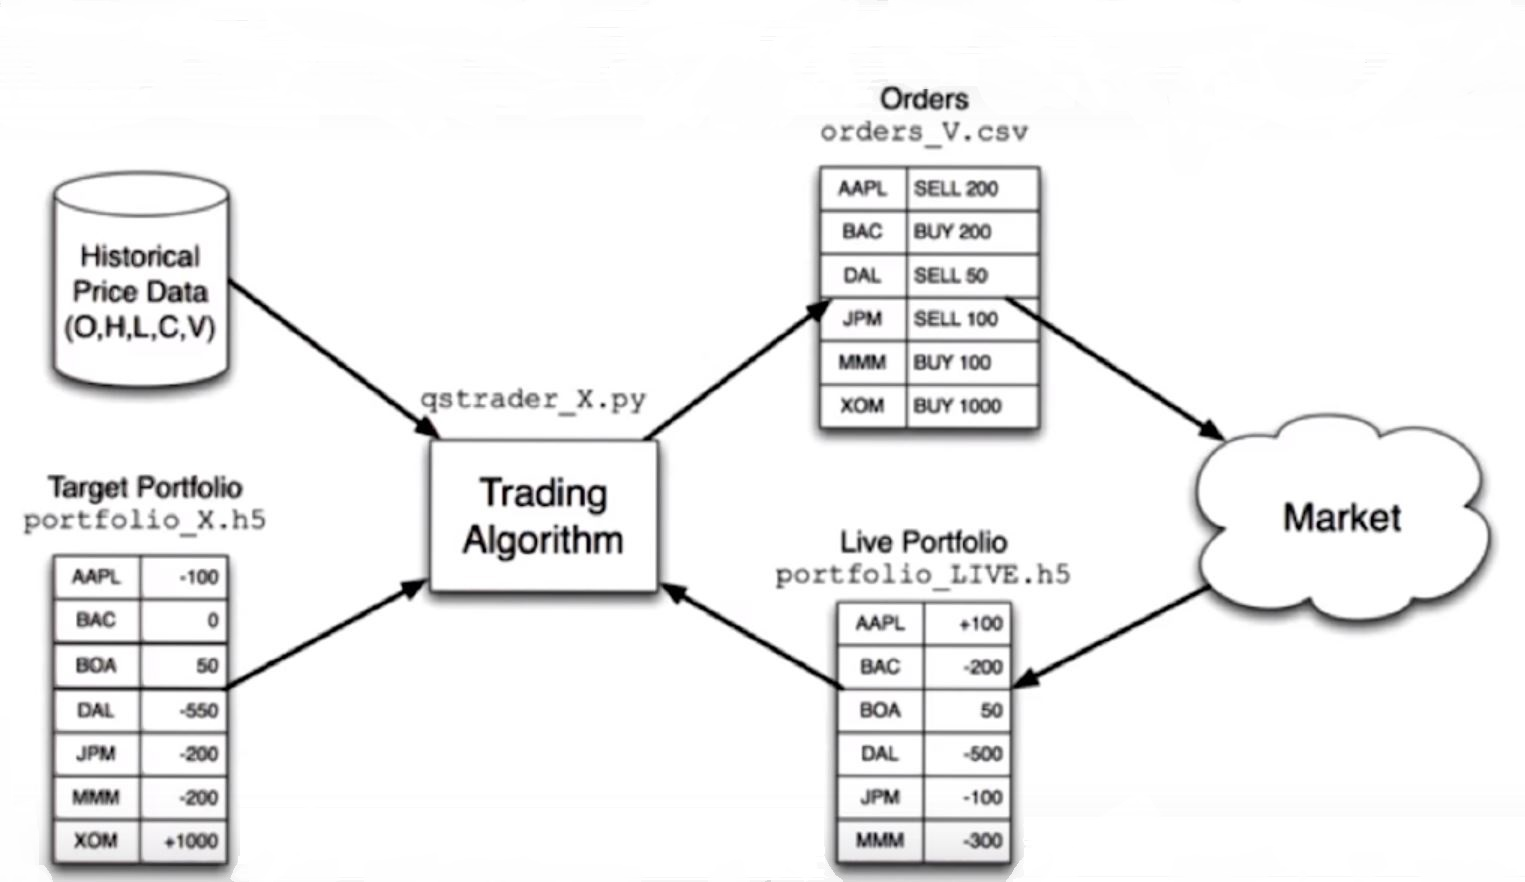
\includegraphics[scale=.4]{images/operation.JPG}
\caption{Graphical representation of hedge fund operation.}
\end{center}
\end{figure}

Trading algorithms work to place certain orders at the proper time. For example, an order for everything in the target portfolio shouldn't be placed all at once because the price of the stock will go up and more money is spent than if strategic ordering were implemented. Additionally, there is another set of computational structures for determining the target portfolio.

\begin{figure}[h!]
\begin{center}
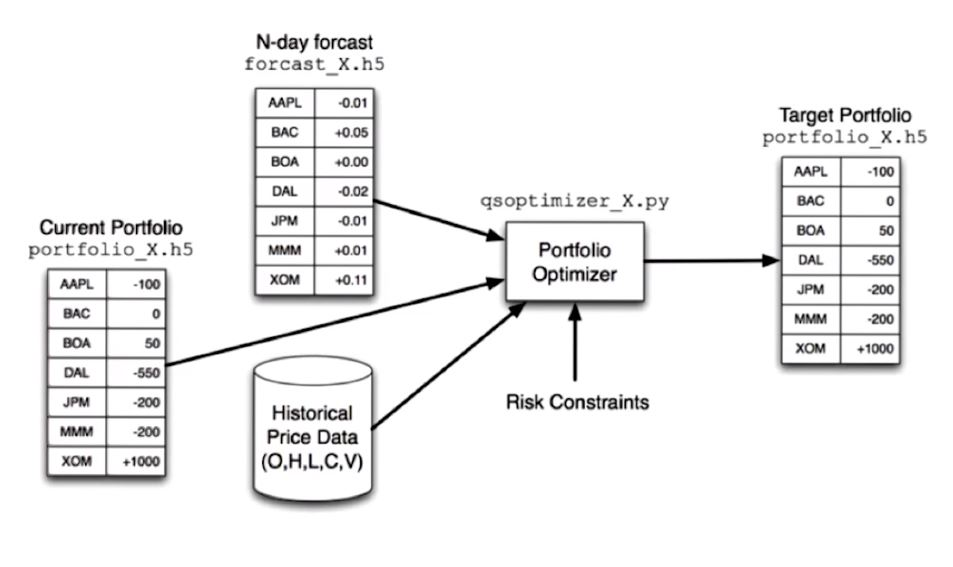
\includegraphics[scale=.75]{images/target.JPG}
\caption{Producing a target portfolio.}
\end{center}
\end{figure}

Historical data, current portfolio, and prediction algorithms are fed into an optimization program to produce a target portfolio. The majority of machine learning comes into play when determining the market forecast. 

\section{Market Mechanics}

\subsection{Ordering}
The live portfolio is altered by giving orders to a broker in the stock market, so it serves to know what exactly is in an order. The broker needs to know whether to buy or sell and of which stock(s) by their market symbols. The order must also contain the number of shares and the type of order. Stock exchanges only consider limit orders and market orders, but note that orders can be increasingly complex based on instructions given to a broker. A market order is an order at the current market price, and ordering at a limit price tells the broker to only buy or sell at a certain price; for example, some may not want to buy beyond some value or sell below some price. Of course, a limit order must also include the desired price. \\

\begin{table}[h!]
\centering
\begin{tabular}{c|c|c|c|c}
BUY/SELL & SYMBOL & SHARES & TYPE & PRICE \\
\hline
BUY & IBM & 100 & MARKET & - \\
BUY & AAPL & 500 & LIMIT & 100 \\
SELL & FB & 1000 & LIMIT & 110 \\
BUY & GOOG & 100 & LIMIT & 740 \\
SELL & NFLX & 50 & MARKET & - \\
SELL & GE & 50 & LIMIT & 40 \\
\end{tabular}
\caption{Example list of orders.}
\end{table}

After the broker sends the order to the stock exchange, it is made public in the style of an "order book". Others can see the stocks and collective bids that have been made on them, but not who has placed the orders. The order book contains a list for each stock of the orders within it including whether the order asks for others to buy or bids on the stock. Both types include a price at which orders are allowed to be bought/sold at and the size of the order. Orders of the same type and price are lumped together. Market orders always sell at the highest bid and buy at the lowest asking price. \\

\begin{table}[h]
\centering
\noindent\begin{tabular}{c@{}l}
  \begin{tabular}{c|c|c}
  	BID/ASK & PRICE & SIZE \\
    \hline
    ASK & 100.10 & 100 \\
	ASK & 100.05 & 500 \\
	ASK & 100.00 & 1000 \\
	BID & 99.95 & 100 \\
	BID & 99.90 & 50 \\
	BID & 99.85 & 50 \\
  \end{tabular} 
  & 
  $\begin{array}{l}
  \\
    \MyLBrace{5ex}{SELL} \\ 
    \MyLBrace{5ex}{BUY} \\ 
  \end{array}$
\end{tabular}
\caption{Example order book.}
\end{table}

The example order book suggests that the price of the stock will decrease because there is much more selling pressure- more are selling than buying. \\

\subsection{Dynamics of Exchange}
There are many stock exchanges, and each has its own order book. When an order is placed, say by an individual, the order is sent to the broker and the broker chooses between the stock exchanges to execute that order. The broker takes information from all the stock exchanges and makes a transaction based on which one has the stock with the best price. Fees are associated with making transactions in stock exchanges and with using a broker. A broker typically has many clients; the broker can observe clients who want to buy and sell at the same price and circumvent stock exchanges entirely. The law ensures that this trade can only happen if both the buyer and seller get prices that are at least as good as at an exchange. Even if this transaction cuts out the stock exchange, it must still be registered with one, and it's usually with the exchange the stock is housed. \\

Orders can be handled internally or moved through what's called a "dark pool". A dark pool is a place where investors can trade without the transparency of an order book outside of a stock exchange. The results of the trade, like internal trades, still need to be registered with public exchanges after they've occured. A dark pool can act as an intermediary between all types of investors that may want to escape the transparency of stock exchanges. Brokers like this because they don't have to pay fees associated with trading at a stock exchange. They also argue that it's fair because clients are getting prices that are as good as at the market. However, hedge funds and dark pools can heavily exploit this system as it stands if they have well-placed, fast computers. \\

\subsection{Exploiting the Market}
These days the market is entirely digital and computers automate transactions all across the country. As a result, orders can be processed in fractions of a second, and timing is everything. A hedge fund may pay stock exchanges enough money to house computers very close to the exchanges, which gives them a distinct advantage. For example, let's say that someone places an order for a stock, and it's sent to multiple markets. A hedge fund close to those markets can see that order reach one of them first and buy up that stock from the other exchanges through the high speed infrastructure they have in place. Then when that order reaches other exchanges, the hedge fund has already bought those shares and sells it back at a higher price. This is one of many strategies in \ac{hft} that takes place on the order of milliseconds. \\

This can also happen on an international scale. A hedge fund may have computers collocated with international markets rapidly observing and comparing order books between them. If a difference occurs in a stock between the two markets, all that needs to be done is to sell in the market with a higher price and buy in the market with a lower one. This happens very quickly, so the price of the stock is not very different at different markets. \ac{hft} strategies usually trade high volumes to turn a large profit in small price differences. \\

Those that operate on \ac{hft} strategies can not only manipulate a transparent market, but also a dark one. First, let's explain why someone would want to use a dark pool. For example, an investor who wants to sell a high volume of shares in a transparent market would want to do so in small chunks so as not to upset the price all at once and get less for the shares. However, others will see this and lower their bids knowing that a high volume is to be sold and the investor still gets less for their shares. In a dark pool, others can't see those that want to buy or sell, so the investor may get a better price. There are many ways to exploit a dark pool, but it always stems from information leakage. Knowing the order book of a dark pool means a world of advantage. Dark pool operators or constituents may secretly participate in their own pool or leak information about it to others for a price. The private nature of a dark pool allows those who operate it to make their own rules about who can participate and how trading works. Since information is at the discretion of the operator, it's fairly easy for those with direct access to exploit a dark pool. Those that don't have direct access can "game" the pool by probing it with many small volume orders. This yields some idea of the size and prices of bids, which gamers can exploit by selling when they find the bids are highest and buying when asking is lowest.

\subsection{Other Orders and Shorting}
Although exchanges only take market and limit orders, other orders can be made through a broker. Often a broker implements them for clients without their knowledge to benefit both themselves and the client. The most simple order above a limit order is a stop-loss order. The broker holds stock until the price drops below a certain price, then sells at market price. Similarly, a stop-gain order waits until the price climbs to a point at which the client wants to sell. Slightly more complex is the trailing stop. Here the broker sets a stop-loss criteria trailing a stock that's increasing in price. As the price increases, so does the stop-loss criteria; when that stock starts to decrease, the stop-loss criteria is met and stocks are sold. \\

What if someone wanted to bet that a stock will decrease and still profit? Instead of just selling high and buying low, those stocks can be borrowed and sold, so the value of those stocks is gained at a high point but the stocks are still owed. Then when the price of the stock decreases, the stock can be bought at a lower value, and the shares returned to whom they were borrowed while a profit on the difference was made. This is called shorting. As long as the price of the stock goes down, this is a good strategy; however, if the price goes up, then the difference results in a net loss. \\

\section{Worth}
The price of a company's stock is intended to reflect the value of the company. Ergo, if the price of a company's stock deviates significantly from its predicted value based on the company's predicted worth, then there's a profitable opportunity for when it returns to reflect the company's worth. The value of the company can be estimated several different ways. One way is to estimate its intrinsic value, which is based on the future dividends the company will give; these are annual payments to stockholders. This doesn't really describe what the company has though. The book value of a company is founded in the company's assets like its facilities and resources. A company's market cap is yet another way to estimate a company's worth, and it's easiest to calculate. This is effectively what the stock market thinks what the company is worth and it's the value of a stock multiplied by the total number of stocks. \\
\newpage
Intrinsic value may not make sense if we try to imagine the value of a company that will pay dividends consistently as long as it stands. However, the company can never be 100\% reliable, so the value of its dividends amount to the value of a promise. The promise of some money in a year is worth less than the same amount given right now because of this principle. Thus, the value of a those promised dividends decreases as the time they're promised is longer, so the total value will converge to a calculable value. Similarly, we can calculate the \ac{pv} of a dollar that is promised after a certain time. It makes sense that the \ac{pv} of a dollar promised right now is a dollar, but what about in a year? The \ac{pv} is some fraction of its \ac{fv} based \ac{ir} and the length of time, $t$.
\begin{align*}
PV=\frac{FV}{(1+IR)^t}
\end{align*}
In this way we have a conversion between the present value and future value of some amount of money. The interest rate is also called the discount rate and it reflects the risk involved with investment. A more stable company will have a lower discount rate because they're more reliable. The intrinsic value, $IV$, of a company can be calculated knowing its discount rate and dividend payments by
\begin{align*}
IV=\frac{FV}{IR}
\end{align*}
Thus, if a hypothetical company pays dividends of \$5 a year and has a discount rate of 1\%, then the value of this company is $\$5/0.01=\$500$. Book value of a company is simple to calculate because it is just what the company has versus what the company owes. If a company only has a factory worth \$1 million, a patent worth \$500,000, and a loan of \$200,000, then the company is worth \$1 million $-200,000=\$0.8$ million. The patent is considered an intangible asset and isn't counted in calculating the book value. \\

News about companies can drastically change some of these measures. Investors reflect their opinions on the worth of a company through stocks- if they feel the company is worth less, they will sell and vice versa. Let's say bad news about a company comes up; investors will see that as increased risk in investing in the company. The company will have to increase their \ac{ir} to appease investors and the intrinsic value of the company will reduce. This would also reduce the stock price of the company, which decreases the market capitalization of the company. News can affect singular companies, sectors of business, and the market as a whole depending on the scope of the news. \\

Market strategies are based on deviations in the estimated values of a company. For example, if the intrinsic value of a company drops and the stock price is relatively high given its history, then it would probably be a good idea to short that stock because the price will almost certainly go down. The book value of a company provides somewhat of a minimum for the market cap; that is because if the market cap goes below the book value, then a predatory buyer typically buys the whole company, breaks it apart, and sells its parts for the book value to turn a profit.
\newpage
\section{The Capital Assets Pricing Model}
The \ac{capm} is a model that is used to predict the return of stocks. To understand this model, a portfolio must be understood in more depth. The term portfolio has been used throughout this text, but has yet to be clearly defined; a portfolio is a set of weighted assets, namely stocks. A portfolio is a set of stocks that are weighted by their value, and all the weights add to 1. Some stocks might be shorted, so technically their portfolio value is negative and really the sum of the absolute value of their weights is 1. Mathematically written, where $w_i$ is the weight of a stock in a portfolio
\begin{align*}
\sum_i |w_i|=1
\end{align*}
and the return of the portfolio for a given day is
\begin{align*}
\sum_iw_ir_i
\end{align*}
where $r_i$ is the return for a stock in a day. As an example, lets say a portfolio is composed of two stocks, A and B, and their respective weights are 0.75 and -0.25 because stock B is shorted. Then if on a given day, stock A increases by 1\% and stock B decreases by 2\%, the result is a portfolio return of $(0.75)(0.01)+(-0.25)(-0.02)=1.25\%$. \\

A similar portfolio can be made for entire markets. Although, it's typically limited to an index which includes the largest companies in a market, like the S\&P 500 for the US market. These companies are weighted by their market caps, so a company's weight in the market is approximately that company's cap, $c$, divided by the sum of all caps.
\begin{align*}
w_i=\frac{c_i}{\sum_{j}c_j}
\end{align*}
The \ac{capm} predicts the return on stocks within a certain market with the simple equation\footnote{Functions have dependent variables in brackets because they are discrete; a result of using digital time.}
\begin{align*}
r_i[t]=\beta_i r_m[t]+\alpha_i[t]
\end{align*}
This says that the return of a stock is largely based on the return of the market as a whole, $r_m$. The degree to which a stock is affected is based on that stocks particular $\beta$ value. Fluctuations that deviate from this are represented in the (theoretically) random variable, $\alpha$, which (theoretically) has an expected value of zero. The $\beta$ and $\alpha$ values of a stock are calculated based on the historical data of daily returns. The daily returns of a stock are plotted against that of the market and the slope of the fitted line constitutes the $\beta$ value. The y-intercept and random deviations describe the $\alpha$ value.

\subsection{CAPM and Related Theories}
The nature of \ac{capm} suggests a specific strategy when approaching the market. \ac{capm} says that the relationship of stocks to the market is linear with an average fluctuation of zero from this relationship. This suggests that the best tactic is to simply choose a set of stocks that will perform well with a certain market environment and sit on them. Active management is a way of thinking that believes the $\alpha$ value is not entirely random and can be predicted. This mindset promotes carefully choosing and trading stocks on a regular basis depending on predicted $\alpha$ values. This is the dichotomy between active and passive portfolio management. If we assume that $\alpha$ is entirely random, then the only way we can beat the market is by predicting the return on the market. However, this is not entirely true, and \ac{capm} will be used to eliminate market risk entirely. \\

\ac{capm} gives $\beta$ values to each stock, but there are other theories that say it's more complicated. One of these is the \ac{apt}, which says that there is not a contribution based on the whole market, but based on its sectors. Moreover, a stock is affected by what happens in the ten different sectors of the economy, and the \ac{capm} equation becomes
\begin{align*}
r_i=\sum_j\beta_{ij} r_j[t]+\alpha_i[t]
\end{align*}
where $j$ denotes the different sectors. This provides a more in-depth prediction of stock return.
\subsection{Using the CAPM}
Now we want to use the \ac{capm} to create a lucrative portfolio. If we say that the return on the market can never be predicted, then any component associated with market return is risk. Applying the \ac{capm} equation to get an overall portfolio return yields
\begin{align*}
r_p=\sum_iw_i[\beta_i r_m(t)+\alpha_i(t)]
\end{align*}
The only way to remove the market return component is to choose weights such that $\sum_iw_i\beta_i=0$. At this point it may seem that there will not be an expected return for the portfolio because \ac{capm} predicts $\alpha$ to be random. It is here that the assumptions of \ac{capm} are wrong. Using some information, we can predict whether a stock will perform better or worse than the market, which will yield a profit regardless of which way the market goes. This information can come from expertise, some analysis, or, in our case, machine learning.

\section{Technical Analysis}
There are effectively two kinds of analysis: fundamental and technical. Fundamental analysis looks at the properties of a company to determine market decisions. Technical analysis looks at patterns in stock prices to make market decision; since technical analysis is clearly more useful aside from predatory buying, that's what will be discussed. \\

Technical analysis only focuses on stock price and volume. Using these to calculate statistics gives indications on what economic decisions to make. Technical analysis is most useful on shorter time scales and when combinations of indicators point to the same decision. \ac{hft} trade at the millisecond timescale and fundamental analysis firms operate at the timescale of years; humans and computers tend to work together at a timescale in between. 
\newpage

\subsection{Some Good Indicators}
It's useful to develop strategies based on time-series indicators, so here are a few. Momentum is a scale dependent indicator that suggests an upward or downward trend depending on slope. Moreover, an $n$-day momentum, $m$, for a stock with price function, $p[t]$, is calculated as
\begin{align*}
m=\frac{p[t]-p[t-n]}{p[t-n]}=\frac{p[t]}{p[t-n]}-1
\end{align*}
This is simply the difference in price as a ratio to the price $n$ days ago. Typically 5, 10, or 20 day momentum is used with values ranging from -0.5 to 0.5. Another indicator is a \ac{sma}; \ac{sma} is also scale dependent looking over an $n$-day window. The price of a stock over $n$ days is averaged and plotted over time where points are placed at the leading end of the window. However, to get a useful value, this needs to be compared to the real time price. Like momentum, it is done as a ratio
\begin{align*}
{SMA}[n]=\frac{p[t]-E(p[t-n:t])}{E(p[t-n:t])}=\frac{p[t]}{E(p[t-n:t])}-1
\end{align*}
Momentum and \ac{sma} together often prove to be strong indicators. For example, if there is strong positive momentum and a crossing of the price from the price being lower than the average to above- this is a good indicator the price will increase. Larger than normal deviations from the moving average are expected to return back to the average and indicate opportunities. Thus, if \ac{sma} is positive, it's a selling opportunity, and a buying opportunity if \ac{sma} is negative. \\

How those decision are made depends on the state of the stock, or its volatility. The standard deviation of the stock's fluctuations provides an excellent measure for when to make decisions. It depends on how certain we want to be that the price is an outlier. The farther the decision threshold is from the \ac{sma}, the more certain we are that the price is an anomaly. From basic statistics, if the decision threshold is placed two standard deviations away from the \ac{sma}, then we are 95\% sure the price is an anomaly. These bands, typically at two standard deviations away from \ac{sma}, are called Bollinger bands. The way this is written mathematically is, again, a ratio, which is between the price difference and the 2$\sigma$ length where $\sigma$ is the standard deviation.
\begin{align*}
{BB}[t]=\frac{p[t]-{SMA}[t]}{2\sigma}
\end{align*}
When making economic decisions, a Bollinger band value greater than 1 denotes a selling opportunity, and less than -1 denotes a buying opportunity. However, it's better to trade when the price crosses the band for the second time because that signals the price moving in a profitable direction. \\

When using these values in a machine learner, it's important that indicators are normalized. To normalize values, follow
\begin{align*}
normal=\frac{value-mean}{\sigma}
\end{align*}
This provides a z-score by which to compare everything.

\subsection{Adjusted Price}
Analysis of historical data is crucial for determining patterns and making economic decisions, but some things drastically  change the price of stocks without having any effect on the real value of the stock. Dividends and stock splits are two things that do just that. The adjusted price accounts for these events and corrects the computational problems that would occur if only the price were taken into account. \\

Stock splits occur when the price of a stock is too high and the company decides to cut the price, but increase the volume so that the overall market cap is the same. This is a problem when dealing with data because it's seen as a large drop in price. The adjusted price is calculated going backwards in time; moreover, the given and adjusted price are the same for a certain starting present day and adjusted going backward in time. If the price is ever split, say by 3, then at the time of the split, the price is divided by 3 so that there is no discontinuity. \\

At the time a company announces the date for payment of dividends, the price of the stock will increase by the amount of a dividend until they're paid at which point the price rapidly decreases by that amount. This is adjusted looking back in time, and on the day a dividend is paid, the prices preceding are decreased by the proportion of the dividend payment. \\

As a note for machine learning, the data that is chosen for the learner is very important. If the stocks from today are chosen and analyzed starting from 7 years ago, then those stocks will of course do well because they've survived. That's using a biased strategy, so what needs to be done is to take index stocks from 7 years ago and run with those. For adjusted price, it's also important to note that the adjusted price will be different depending on where the starting point is chosen, and that should also be taken into account.

\section{Efficient Markets Hypothesis}
\noindent Until now, we've been assuming, for technical analysis, that there is information in historical data that we can exploit to determine what the market is going to do. The same goes for fundamental analysis in terms of fundamental data. However, the Efficient Markets Hypothesis says that we're wrong on both accounts!\\

\noindent Here are some assumptions of the Efficient Markets Hypothesis:

\begin{enumerate}
	\item \textbf{Large number of investors} The most important assumption of EMH is that there are a large number of investors for-profit. They have incentive to find where the price of a stock is out of line with its true value. Because there are so many investors, any time new information comes out, the price is going to change accordingly.
    
    \item \textbf{New information arrives randomly} 
    \item \textbf{Prices adjust quickly}
    \item \textbf{Prices reflect all available information}
\end{enumerate}

\subsection{The three forms of the EMH}
\noindent There are 3 forms of the EMH, ranging from weak to strong.

\paragraph{Weak} Future prices cannot be predicted by analyzing historical prices. This leaves room for fundamental analysis, however.
\paragraph{Semi-strong} Prices adjust rapidly to new public information
\paragraph{Strong} Prices reflect all information, public and private
\subsection{Is the EMH correct?}
\noindent If the EMH is correct, a lot of what we're trying to do is impossible, so we should cut our losses and go home. Luckily, there is evidence for why certain versions of the hypothesis are incorrect. The existence of hedge funds indicates that you can profit by investing in stocks other than the market portfolio.\\

\noindent The strong version is the weakest of the three, considering there are many examples of insiders using esoteric information for their own benefit. And in many cases, these people have gone to jail!\\

\noindent There is also data that shows that the semi-strong version isn't too likely to be correct. You can see trends in 20-year annualized returns versus 10-year P/E ratio data, which means that you most likely can use fundamentals to predict future performance.\\

\section{The Fundamental Law of Active Portfolio Management}
\noindent Richard Grinold was trying to find a way of relating performance, skill, and breadth. For example, you might have lots of skill to pick stocks well, but you might not have the breadth to use that skill. So he developed the following relationship:
\begin{equation*}
{performance} = {skill}\sqrt{breadth}
\end{equation*}

\noindent So we need some way of measuring skill and breadth. Performance is summarized by something called the \textit{information ratio}:

\begin{equation} \label{eq:inforatio}
{IR} = {IC}\sqrt{BR}
\end{equation}

\noindent where $IC$ is the \textit{information coefficient}, and $BR$ is the number of trading opportunities we have.

\subsection{The Coin-flipping Casino}
\noindent As a thought experiment, instead of buying and selling stocks, we're going to flip coins, and bet on the outcome. This is analogous to buying a stock and holding it-- either you earn or lose money.\\

\noindent The coin is biased (like $\alpha$) to $P(heads) = .51$. The uncertainty of the outcome is like $\beta$.

\paragraph{Betting} Betting works by betting on $N$ coins. If we win, we now have $2N$ coins. If we lose, we now have $0$ coins, so this is an even-money bet (you either gain $N$ coins or lose $N$ coins.)

\paragraph{The Casino} The casino has 1000 tables, each with a biased coin, and you have 1000 tokens, so you can bet them in any way you like: 10 tokens each on 100 tables, 1 token on each table, or 1000 tokens on 1 table. Once bets have been placed, the coins are all flipped in parallel, and for each game you either lose your chips or win.

\noindent So now the question is what scenario is going to net you the best outcome? Let's take the following two bets for example:

\begin{enumerate}
\item 1000 tokens on one table and 0 on the other 999
\item 1 token on each of 1000 tables
\end{enumerate}

\noindent Which is better? Or are they the same? In fact, the expected return of both bets are the same, but bet 2 is much less risky, as with bet 1, if you lose, you lose all of your money, but with bet 2, you might lose around half your money. In fact, the chance of losing all of your money (if you bet tails) is:

\begin{equation*}
(.49)^{1000} \approx 10^{-310}
\end{equation*}

\noindent To determine which is best, we need to consider risk and reward. In this case, the reward is our expected return. If $P_w$ is the chance we would win, and $P_l$ is the chance that we would lose, and $W$ is the amount we would win, whereas $L$ is the amount we'd lose, expected return for a single bet is calculated as follows:

\begin{equation*}
	E[R] = P_wW + P_lL
\end{equation*}

\noindent For the biased coin where we place all of our bets on one table, this would be:

\begin{equation*}
	E[R] = .51(\$1000) + .49(-\$1000) = \$20
\end{equation*}

\noindent If we placed 1 token on each table, the expected return would be:

\begin{equation*}
	E[R] = \sum_{i=1}^{1000} .51(\$1) + \sum_{i=1}^{1000} .49(-\$1) = \$20
\end{equation*}

\noindent So, in terms of reward, neither is better or worse. So how do we choose how to allocate the tokens? It turns out that the risk makes it easy to choose.\\

\noindent First, what's the chance that we lose it all? For the case where all of our tokens are on one table, the chance is 49\%. For the second table, it's around $10^{-308}\%$, which is quite a bit smaller...\\

\noindent Another way to look at the risk is by looking at the standard deviation of the bets. An example of the outcomes for situation 2 is:

\begin{equation*}
	-1,1,1,1,-1,-1,1,-1,...,1
\end{equation*}

\noindent The standard deviation of which is just 1. Now, for the case where we put all of our tokens on one table, the outcomes look like this:

\begin{equation*}
	1000,0,0,0,0,...,0
\end{equation*}
or
\begin{equation*}
	-1000,0,0,0,0,...,0
\end{equation*}

\noindent The standard deviation (risk) in both cases is $\sqrt{1000} \approx 31.62$, which is much higher than the standard deviation for putting bets on each table.

\noindent Now, we can create a risk-adjusted reward (Sharpe Ratio) for the single-bet case:

\begin{equation*}
	R_{s} = \frac{\$20}{\$31.62} = 0.63
\end{equation*}

\noindent For the multi-bet scenario, it's:

\begin{equation*}
	R_{m} = \frac{\$20}{\$1} = 20.0
\end{equation*}

\noindent Clearly, the second case wins based on this ratio. Something interesting about these results is that:

\begin{equation*}
	20 = .63\sqrt{1000}
\end{equation*}
\noindent It turns out that this can be generalized to 

\begin{equation*}
	{SR}_{multi} = {SR}_{single}\sqrt{bets}
\end{equation*}

\noindent Which shows that as we increase the number of bets (diversify), the Sharpe Ratio increases. This is the relationship described in the Fundamental Law of Active Portfolio Management; to increase performance, you can either increase skill or diversify (bets), although diversification only goes as the square root.\\

\noindent Now, back to equation~\ref{eq:inforatio}. Let's define what \textit{information ratio} means. If we consider the CAPM equation:

\begin{align*}
r_p[t]=\beta_p r_m[t]+\alpha_p[t]
\end{align*}

\noindent we can associate the first term, $\beta_p r_m[t]$ with the market, and the second term, $\alpha_p[t]$ with skill. Information ratio is defined as:

\begin{equation} \label{eq:inforatiodef}
IR = \frac{\overline{\alpha_p[t]}}{\sigma_{\alpha_p[t]}}
\end{equation}

\noindent Information ratio can be thought of as a Sharpe Ratio of excess return (due to skill). Now, the \textit{information coefficient}, $IC$, is the correlation of forecasts to returns. $IC$ can range from 0 (no skill) to 1 (perfect skill). $BR$, or breadth, is the number of trading opportunities per year. For example, if you are Warren Buffet, and hold only 120 stocks for a whole year, $BR$ is just 120. However, if you have 120 stocks and trade them daily, $BR = 120*365$.\\

\noindent Let's do an example: say that James Simons and Warren Buffet both have the same information ratio, and that Simons' algorithm is 1/1000 as smart as Buffet's. Buffet only trades 120 times per year. How many trades per year must Simons execute to have the same information ratio (performance)?

\begin{align*}
IR_S &= IC_S\sqrt{BR_S}\\
IR_B &= IC_B\sqrt{BR_B}\\
IC_S &= 1/1000IC_B\\
\frac{IR_B}{IR_S} &= \frac{IC_S\sqrt{BR_S}}{IC_B\sqrt{BR_B}} = 1\\
&= \frac{\frac{1}{1000}\sqrt{BR_S}}{\sqrt{BR_B}}\\
&\Rightarrow BR_S = (1000)^2BR_B\\
&= 120,000,000
\end{align*}

\noindent So Simons must execute 120 million trades, whereas Buffet only needs to execute 120. That's quite a difference! Indeed, skill is an extremely important factor in performance.

\section{Portfolio Optimization}
Now we wish to optimize a portfolio, and what this means is minimizing risk for a given target return. Risk is largely defined as the volatility of a stock. A portfolio is composed of some stocks that individually have their own return-risk ratios, but it is possible to weight them such that the return-risk ratio of the portfolio is higher than that of any individual stock. \\

This is done through combining correlated and anti-correlated stocks to highly reduce volatility. In the case of a highly correlated group of stocks, their combination results in a similar volatility, but if they're combined with highly anti-correlated stocks, then with accurate weighting, fluctuations cancel out and volatility is minimal while yielding similar returns. A useful algorithm to find the best weighting is \ac{mvo}. \textbf{*This algorithm is not explained, but we should find it*}. \ac{mvo} and similar algorithms find the minimal risk for a given target return, and if this is plotted over all target returns, we get a curve called the efficient frontier. On a return-risk plot, a line tangent to the efficient frontier with an intercept at the origin also points to the portfolio with the minimal Sharpe ratio.

\chapter{Machine Learning Algorithms}
\noindent In most cases, machine learning algorithms are focused on building a model. Then, the model can be used to take inputs and give outputs based on the model. The model is a tool to predict outputs based on the inputs. In our case, we will be using models to take information about stocks and predict their future prices.
\begin{figure}[h]
\centering
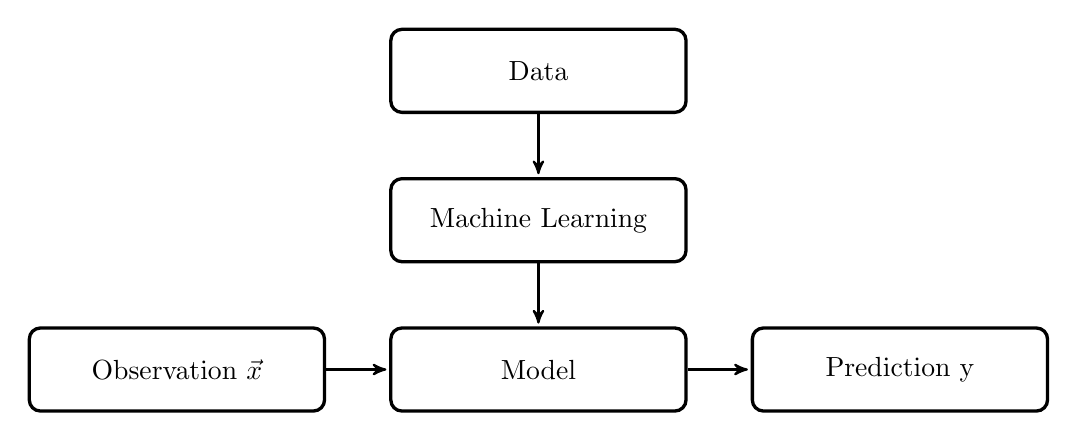
\begin{tikzpicture}
  [node distance=.8cm,
  start chain=going below,]
  	\node (data) [punktchain] {Data};
    \node (ml) [punktchain, join=by {->}] {Machine Learning};
      \node (model) [punktchain, join=by {->}]  {Model};
      \begin{scope}[start branch=venstre,
        %We need to redefine the join-style to have the -> turn out right
        every join/.style={->, thick, shorten <=1pt}, ]
        \node[punktchain, on chain=going left, join=by {<-}]
            (inputs) {Observation $\vec{x}$};
      \end{scope}
      \begin{scope}[start branch=hoejre,]
      \node (finans) [punktchain, on chain=going right, join=by {->}] {Prediction y};
    \end{scope}
  % Now that we have finished the main figure let us add some "after-drawings"
  %% First, let us connect (finans) with (disk). We want it to have
  %% square corners.
\end{tikzpicture}
\end{figure}

\noindent So we use machine learning to take historical data and generate a model. When we want to use it, we give the model observations, $\vec{x_i}$, and it gives us predictions, $y$. Examples of good inputs (predictive factors) are:
\begin{enumerate}
	\item Price momentum
    \item Bollinger value
    \item Current price
\end{enumerate}
\noindent while examples of outputs would be:
\begin{enumerate}
	\item Future price
    \item Future return
\end{enumerate}
\noindent We'll first talk about Supervised Regression Learning.

\section{Regression and Modeling}
\noindent Supervised Regression Learning means that we'll provide (supervised learning) a bunch of example data $(x,y)_i$ and allow the model to make a numerical prediction (regression). There are two main types of regression techniques:
\begin{itemize}
\item Linear regression (parametric)
\item \ac{kNN} (instance-based), the more popular approach
\item Decision trees
\item Decision forests
\end{itemize}

\section{Assessing a Model}
Assessing a model is much like predicting prices as it uses indicators to judge the effectiveness of the model. The first indicator is \ac{rmse}, which is as follows
\begin{align*}
\sqrt{\frac{\sum(y_{test}-y_{predict})^2}{N}}
\end{align*}
The error that is important is that of test data, which is outside of the training data. Typically 60\% of the data is used for training, and 40\% is used for testing. However, sometimes there isn't enough data to adequately evaluate a learning algorithm, in which case a method called \textbf{cross validation} is used. This method slices the data into chunks, typically fifths. One is chosen as test and the rest are for training, then a different chunk is chosen to be the test and another trial is run. For financial data, we don't want to accidentally look forward in time, so we would only use \textbf{roll forward cross validation}. This simply demands that all the training data is before the test data. \\

The second metric for how well an algorithm is working is the \textbf{correlation} of the test data and predicted values. Strong correlation, close to $\pm$1, indicates a good algorithm whereas a weak correlation, close to zero, indicates a poor algorithm. Correlation and \ac{rmse} are excellent indicators on how well an algorithm is doing, but we might also want to fine tune an algorithm; we want to answer the question "when are we trying too hard to fit data?". This is where \textbf{overfitting} comes into play. Overfitting is the point at which error for training data is decreasing while error for test data is increasing.
\begin{figure}[h]
\centering
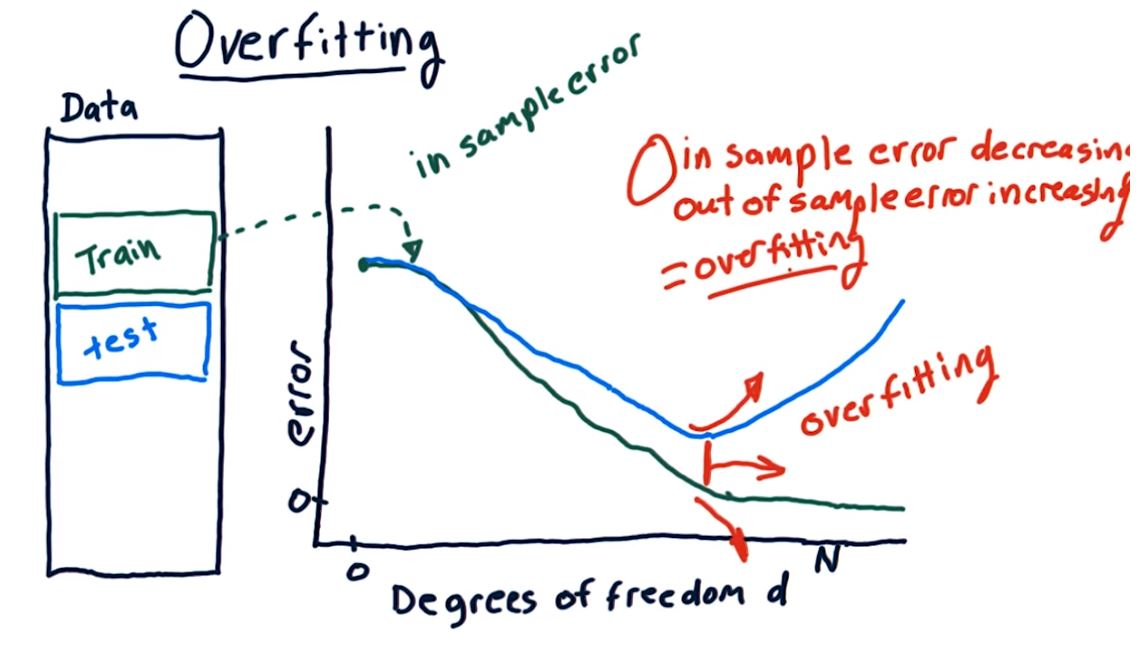
\includegraphics[scale=.6]{images/overfit.JPG}
\end{figure}

\section{Types of Learners}

\paragraph{Ensemble Learners}
Ensemble learners are composed of several different learners, which could include \ac{kNN}, regression, and decision tree learners in one. The output of this learner is then simply a combination of the learners' answers, which is typically an average of the outputs.

\paragraph{Bagging and Boosting}
Boot-strap aggregating, or \textbf{bagging}, only uses one algorithm, but many different models. If the training data is separated into learning instances where there's a total of $n$ instances, then each model is fed a bag of these instances. Each bag is composed of $n'$ learning instances that are randomly selected with replacement, so instances may show up more than once in the same bag. These are used to train $m$ models and the result is the average of all the outputs. \textbf{Boosting} builds each subsequent bag based on the results of the last. Training data is also used to test the models, and a model's predicted data showing significant error is weighted to more likely be in the next bag for the next model. The process is continued for the desired number of models, and the results are averaged. Although this could be advantageous in predicting outliers, it's also more susceptible to overfitting.

\subsection{Reinforcement Learning}
As seen in figure 4.1, reinforcement learning describes the interaction of a robot with its environment. The robot performs an action, which has an effect on the environment and changes its state. The robot observes the change in state and its associated reward and makes decisions to maximize that reward.

\begin{figure}[h]
\centering
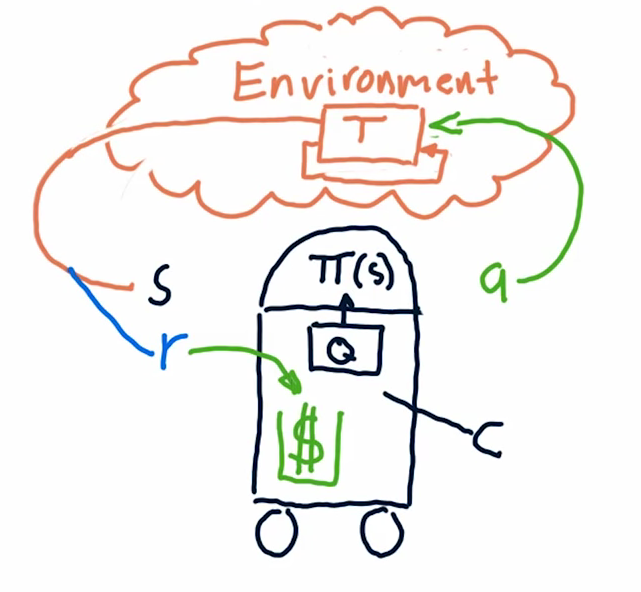
\includegraphics[width=6cm]{images/rl.png}
\caption{A diagram of how policy learning works}
\end{figure}

Reinforcement learning also describes the problem that is how to go about maximizing the reward. In the stock market, the reward is return on trades, and we want to find out how to maximize returns. This problem is complicated by time constraints. The value of future gains diminishes with time, so it's unreasonable to use an infinite horizon on which to base returns. However, optimizing returns over too short a time may limit rewards from seeing a much larger overall gain.

\subsection{Markov Decision Problems}
\noindent What we've been talking about is called a Markov decision problem. Here's how the problem is formalized.

We have:
\begin{itemize}
\item Set of states $S = \{s_1, \ldots, s_n\}$
\item Set of actions $A = \{a_1, \ldots, a_n\}$
\item Transition function $T[s,a,s']$
\item Reward function $R[s,a]$
\end{itemize}

\noindent What we're trying to find is a policy $\pi(s)$ that will maximize the reward. Unfortunately, we don't know the $T$ or $R$, since that's defined by the environment. So, the learner has to interact with the world and see what happens. Based on the reward, it can start generating policies.\\

\noindent A way to encode this information is using \textbf{experience tuples}. Experience tuples are as follows: given a state $s_1$ and an action $a_1$ that we took, we were put into state $s_1'$ and got reward $r_1$. The tuple is shown like this:

\begin{equation*}
\langle s_1, a_1, {s_1}', r_1 \rangle
\end{equation*}

\noindent Now, we can rename ${s_1}'$ to $s_2$, since that's our new state, and then take a new action and see what happens, and we get a new tuple:
\begin{equation*}
\langle s_2, a_2, {s_2}', r_2 \rangle
\end{equation*}

\noindent And we repeat this for many different combinations of states and actions, and then we'll use the tuples to generate the policy. There are two ways to generate the policy:

\paragraph{Model-based} For this method, we generate a model of $T[s,a,s']$ based on statistical analysis of the tuples. We look at a particular state and a particular action and see the probability of transitioning to another state. Same thing with $R[s,a]$. Then, we can use policy or value iteration to solve it.

\paragraph{Model-free} This method keeps the data around and uses the original tuples to determine what the new state will be for a certain action. This is Q-learning.

\section{Q-Learning}

\noindent Q-Learning is a model-free approach, which means that it doesn't need to have any sort of model of the transition function $T$ or the reward function $R$. It builds a table of \textit{utility values} as the agent interacts with the world. These are the Q values. At each state, the agent can then use the Q values to select the best action. Q-Learning is guaranteed to give an optimal policy, as it is proven to always converge.\\

\noindent Q represents the \textit{value} of taking action $a$ in state $s$. This value includes the immediate reward for taking action $a$, and the discounted (future) reward for all optimal future actions after having taken $a$. \\

\subsection{How do we use Q?}
\noindent What we want to find for a particular state is what policy, $\Pi(s)$ we should take. Using Q values, all we need to do is find the maximum Q value for that state.

\begin{equation}
\Pi(s) = {argmax}_{a}(Q[s,a])
\end{equation}

\noindent So, we go through each action $a$ and see which action has the maximum Q value for state $s$. Eventually, after learning enough, the agent will converge to the optimal policy, $\pi^*(s)$, and optimal Q table, $Q^*[s,a]$.

\subsection{How do we get Q?}
\noindent To use the Q table, first we must generate it by learning. How do we go about that? Well it's similar to previous learning algorithms, in that we provide it training data for which we know the outcomes. We then iterate over time and take actions based on the current policy ($Q$ values), and generate experience tuples $\langle s,a,s',r\rangle$ and generate the $Q$ values based on the experience.\par

\noindent In a more detailed fashion:

\begin{enumerate}
\item Initialize the $Q$ table with small random values
\item Compute $s$
\item Select $a$
\item Observe $r, s$
\item Update $Q$
\item Step forward in time, then repeat from step 2.
\end{enumerate}

\noindent To update $Q$, we first need a formula to decide what it should be. What we can do is assign a \textit{learning rate}, $\alpha$, to weight the new observations. We can therefore update $Q$ like this:

\begin{equation*}
Q'[s,a] = Q[s,a] + \alpha({improved\ estimate} - Q[s,a])
\end{equation*}

\noindent As you can see, $Q$ converges as the improved estimate is the same as the current estimate (we're at the best $Q$). Now, we need to know what the improved estimate is:

\begin{equation*}
improved\ estimate = immediate\ returns + (discounted\ future\ rewards)
\end{equation*}

\noindent Then, replacing \textit{discounted future rewards} with the actual way of calculating it, and rearranging to only use the current value of $Q$ once, we find that the formula to calculate the new value of Q for a state-action pair $\langle s,a\rangle$, the formula is:

\begin{equation}
Q'[s,a] = (1-\alpha)Q[s,a] + \alpha (r+\gamma\ Q[s',{argmax}_{a'}(Q[s',a'])])
\end{equation}

\noindent where:
\begin{itemize}
\item $r = R[s,a]$ is the \textit{immediate reward} for taking an action $a$ in the state $s$
\item $\gamma \in [0,1]$ is the \textit{discount factor} to reduce the value of future rewards
\item $s'$ is the resulting next state
\item ${argmax}_{a'}(Q[s',a'])$ is the action which maximizes the Q-value among all possible actions $a'$ from $s'$, and
\item $\alpha \in [0,1]$ is the \textit{learning rate} used to vary the weight given to new experiences compared to past Q-values. It's typically around 0.2.
\end{itemize}

\subsection{Exploration}
\noindent The success of a Q-learning algorithm depends on the exploration of the state-action space. If you only explore a small subset of it, you might not find the best policies. One way to ensure that you explore as much as possible is to introduce randomness into selecting actions during the learning phase. So basically, you see first whether you want to take the action with the maximal Q value or choose a random action, then if you take a random action, each action gets a probability which decreases over subsequent iterations.

\subsection{Q-Learning for Trading}
\noindent Now that we know what Q-learning is, we need to figure out how to apply it to the context of trading. That means that we need to define what \textit{state}, \textit{action}, and \textit{reward} mean. Actions are straightforward, as there are basically three of them:

\begin{itemize}
\item {\color{DarkerGreen} BUY}
\item {\color{red} SELL}
\item NOTHING
\end{itemize}

\noindent Our rewards can be daily returns or cumulative returns after a trade cycle (buy$\rightarrow$sell). However, using daily returns will allow the agent to converge on a $Q$ value more quickly, because if it waited until a sell, then it would have to look at all of the actions backwards until the buy to get that reward.\\

\noindent Now, we just need to figure out how to determine state. Some good factors to determine state are:

\begin{itemize}
\item Adjusted Close/Simple Moving Average
\item Bollinger Band value
\item P/E ratio
\item Holding stock (whether or not we're holding the stock)
\item Return since entry
\end{itemize}

\noindent Our state must be a single number so we can look it up in the table easily. To make it simpler, we'll confine the state to be an integer, which means we need to discretize each factor and then combine them into an overall state. Our state space is discrete, so the combined value is the overall state. Say we have a state like this:

\begin{table}[h]
\centering
\begin{tabular}{ccc}
\textbf{Factor} & \textbf{Value} & \textbf{Discretized}\\
$X_1$ & 25.6 & 0\\
$X_2$ & 0.3 & 5\\
$X_3$ & 2.0 & 9\\
$X_4$ & -5.1 & 2
\end{tabular}
\end{table}

\noindent The discretized state could be: 2950.

\paragraph{Discretization} To discretize, what we do is take the data for a factor over its range, then divide it into $n$ bins. Then we find the threshold by iterating over the data by the step size and taking the value at each position.

\begin{lstlisting}[style=python]
stepsize = size(data)/n
data.sort()
for i in range(0, steps):
	threshold[i] = data[(i+1)*stepsize]
\end{lstlisting}

\begin{figure}[h]
\centering
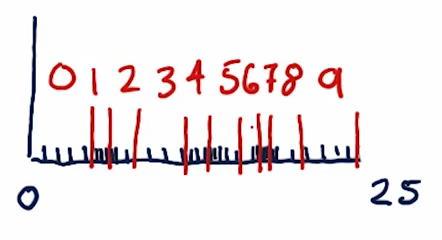
\includegraphics[width=6cm]{images/discretization.png}
\caption{What the thresholds might look like for a discretized data set if $n = 10$}
\end{figure}

\subsection{Problems with Q-Learning}
\noindent One main problem with Q-Learning is that it takes a lot of experience tuples to converge to the optimal Q value. This means the agent has to take many \textit{real} interactions with the world (execute trades) to learn. The way this has been addressed is by using \textit{Dyna}.

\section{Dyna-Q}

\noindent Dyna is designed to improve the convergence of Q learning by building a model of $T$ and $R$ and then using Q learning to make decisions based on the model. However, the Q learning portion is still model-free, so it's a mix of both.\\

\noindent So we do the Q-Learning steps, but after we take an action, we update the model of $T$ and $R$ with the new data, simulate a bunch of experiences based on the model, then update $Q$ based on these simulated experiences. To simulate the experiences, we basically generate random states and actions, and then find the new states/rewards based on the transition function and reward function.

\subsection{Learning $T$}

\noindent To figure out a model for T, what we can do is count the number of times that a transition to $s'$ by using the action $a$ in state $s$ occurred, then divide that by the total number of transitions to figure out the probability.

\begin{equation}
T[s,a,s'] = \frac{T_c[s,a,s']}{\sum_{i} T_c[s,a,i]}
\end{equation}

\noindent where $T_c$ is the number of times the transition occurred.

\subsection{Learning $R$}

\noindent To finalize the model, we need to find our expected reward, $R[s,a]$. Whenever we interact with the world, we get an immediate reward, $r$. We can use this to update our model for $R$ in a similar way to updating the Q values.

\begin{equation}
R'[s,a] = (1-\alpha)R[s,a] + \alpha r
\end{equation}

\noindent where $\alpha$ is, again, the learning rate.

\subsection{Conclusion}
\noindent So a summary of how Dyna-Q works is the following:

\begin{align*}
\noindent Q\ learning&\left\{
	\begin{tabular}{@{}l@{}}
    	init Q table\\
        observe S\\
        execute a, observe s;r\\
        update Q with $\langle s, a, s', r \rangle$\\
    \end{tabular}
\right.\\
\noindent Update\ model&\left\{
	\begin{tabular}{@{}l@{}}
    	update T'[s,a,s']\\
        update R'[s,a]
    \end{tabular}
\right.\\
\noindent Dyna\ Q&\left\{
	\begin{tabular}{@{}l@{}}
    	s = random\\
        a = random\\
        s' = infer from $T$\\
        r = R[s,a]\\
        update Q with new experience tuple\\
        repeat many times ($\sim100-200$)
    \end{tabular}
\right.
\end{align*}

\begin{figure}[h]
	\centering
	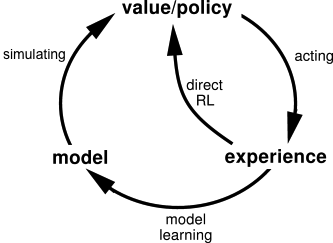
\includegraphics[width=7cm]{images/Dyna-architecture.png}
	\caption{A diagram of the Dyna architecture (courtesy Sutton and Barto)}
\end{figure}
\appendix
\chapter{Additional Code Examples} \label{App:AppendixA}
\section{Statistics}
\subsection{Polynomial Fit}
\begin{figure}[h!]
	\centering
	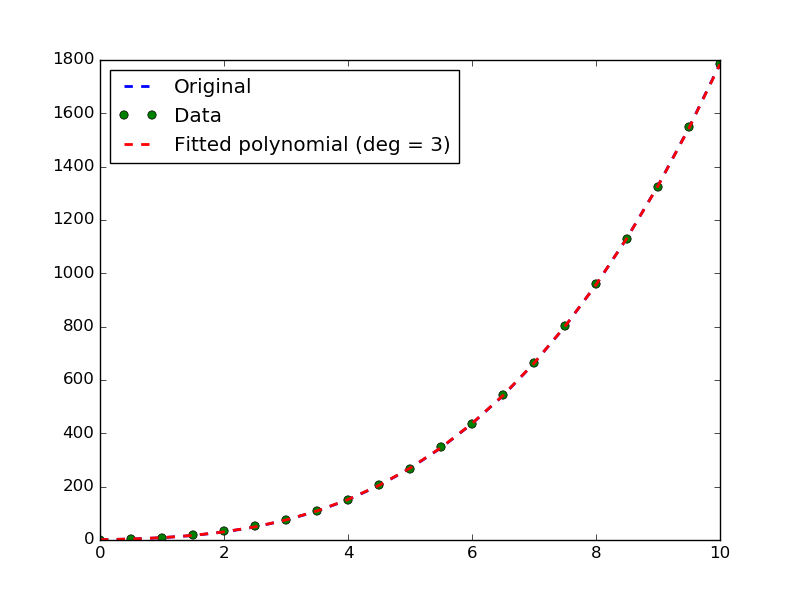
\includegraphics[width=\linewidth]{images/poly_fit.png}
    \caption{Polynomial fit to noisy data}
\end{figure}
\newpage
\noindent\begin{minipage}{\linewidth}
\begin{lstlisting}[style=python]
import pandas as pd
import numpy as np
import matplotlib.pyplot as plt
import scipy.optimize as spo

def error_poly(C,data):
	return np.sum((data[:,1] - np.polyval(C,data[:,0])) ** 2)

def fit_poly(data,error_func,degree=3):
	guess = np.poly1d(np.ones(degree+1, dtype=np.float32))

	return spo.minimize(error_func, guess, args=(data,), method='SLSQP', options={'disp':True}).x

def test_run():
	original_poly = np.float32([1.5,2.5,3.5,1])

	Xoriginal = np.linspace(0,10,21)
	Yoriginal = np.polyval(original_poly,Xoriginal)
	plt.plot(Xoriginal,Yoriginal,'b--',linewidth=2.0,label="Original")

	noise_sigma = 2
	noise = np.random.normal(0,noise_sigma,Yoriginal.shape)

	data = np.asarray([Xoriginal,Yoriginal+noise]).T

	degree = 3
	poly = fit_poly(data,error_poly,degree)

	plt.plot(data[:,0],data[:,1],'go',label="Data")

	plt.plot(data[:,0],np.polyval(poly,data[:,0]),'r--',linewidth=2.0,label="Fitted polynomial (deg = {})".format(degree))
	plt.legend(loc='upper left')
	plt.show()

if __name__ == "__main__":
	test_run()
\end{lstlisting}
\end{minipage}

\section{Algorithms}
\subsection{kNN Learner}
\noindent\begin{minipage}{\linewidth}
\begin{lstlisting}[style=python]
import numpy as np

class KNNLearner(object):
	def __init__(self, k):
		self.k = k
		self.x = None
		self.y = None

	def addEvidence(self, X,Y):
		if(self.x is None):
			self.x = X
			self.y = Y
		else:
			self.x = np.vstack((self.x, X))
			self.y = np.append(self.y, Y)

	def query(self, points):
		ret = np.array([])
		for point in points:
			ret = np.append(ret, self.y[np.linalg.norm(self.x-point,axis=1).argsort()[:self.k]].mean())	# get the k closest x locations, then find the mean of their y values
		return ret
\end{lstlisting}
\end{minipage}

\noindent Running this on some 2-dimensional x testing data, we can compare the linear regression learner to the kNN learner:

\noindent\begin{minipage}{\linewidth}
\begin{lstlisting}[style=python]
==== kNNLearner =====
In sample results
RMSE:  0.293210201429
corr:  0.933616301402

Out of sample results
RMSE:  0.40276819912
corr:  0.867504170015

==== LinRegLearner =====
In sample results
RMSE:  0.515854106381
corr:  0.776302806055

Out of sample results
RMSE:  0.52366864612
corr:  0.758354066174
[Finished in 0.1s]
\end{lstlisting}
\end{minipage}
\noindent The kNN learner was run with $k = 3$.

\subsection{kNN Bag Learner}
\noindent\begin{minipage}{\linewidth}
\begin{lstlisting}[style=python]
import KNNLearner as knn
import numpy as np
import util

class KNNBag(object):
	def __init__(self, k=(3,4)):
		self.bags = [knn.KNNLearner(kN) for kN in k]

	def addEvidence(self, X, Y, n):
		for bag in self.bags:
			rows = np.random.randint(X.shape[0], size=n)
			bag.addEvidence(X[rows,:],Y[rows])

	def query(self, points):
		return np.average(np.array(map(lambda learner:learner.query(points), self.bags)), axis=0)

	def __str__(self):
		bag_string = '\n'.join(map(lambda bag: str(bag).replace('\n','\n\t'), self.bags))
		return "========== kNN Bag Learner ==========\n# Bags: {}\n{}\n=====================================".format(len(self.bags), bag_string)
\end{lstlisting}
\end{minipage}
\end{document}